\documentclass{article}
\usepackage[utf8]{inputenc}
\usepackage{minted}
\usepackage{graphicx}
\usepackage{hyperref}
\usepackage[dvipsnames]{xcolor}


\title{tuto uart idosens}
\author{cmonaton }
\date{September 2019}

\begin{document}

\maketitle

\section{Introduction}
L'objectif est d'utiliser l'UART pour faire communiquer le produit idosens avec le PC.

\subsection{Matériel}
Détécteur d'ouverture de porte idosens :


Pièces détachées :
Base :




%Capteur :

%alimentation :

%télécommande :


\begin{figure}[H]
\begin{center}
\advance\leftskip-3cm
\advance\rightskip-3cm
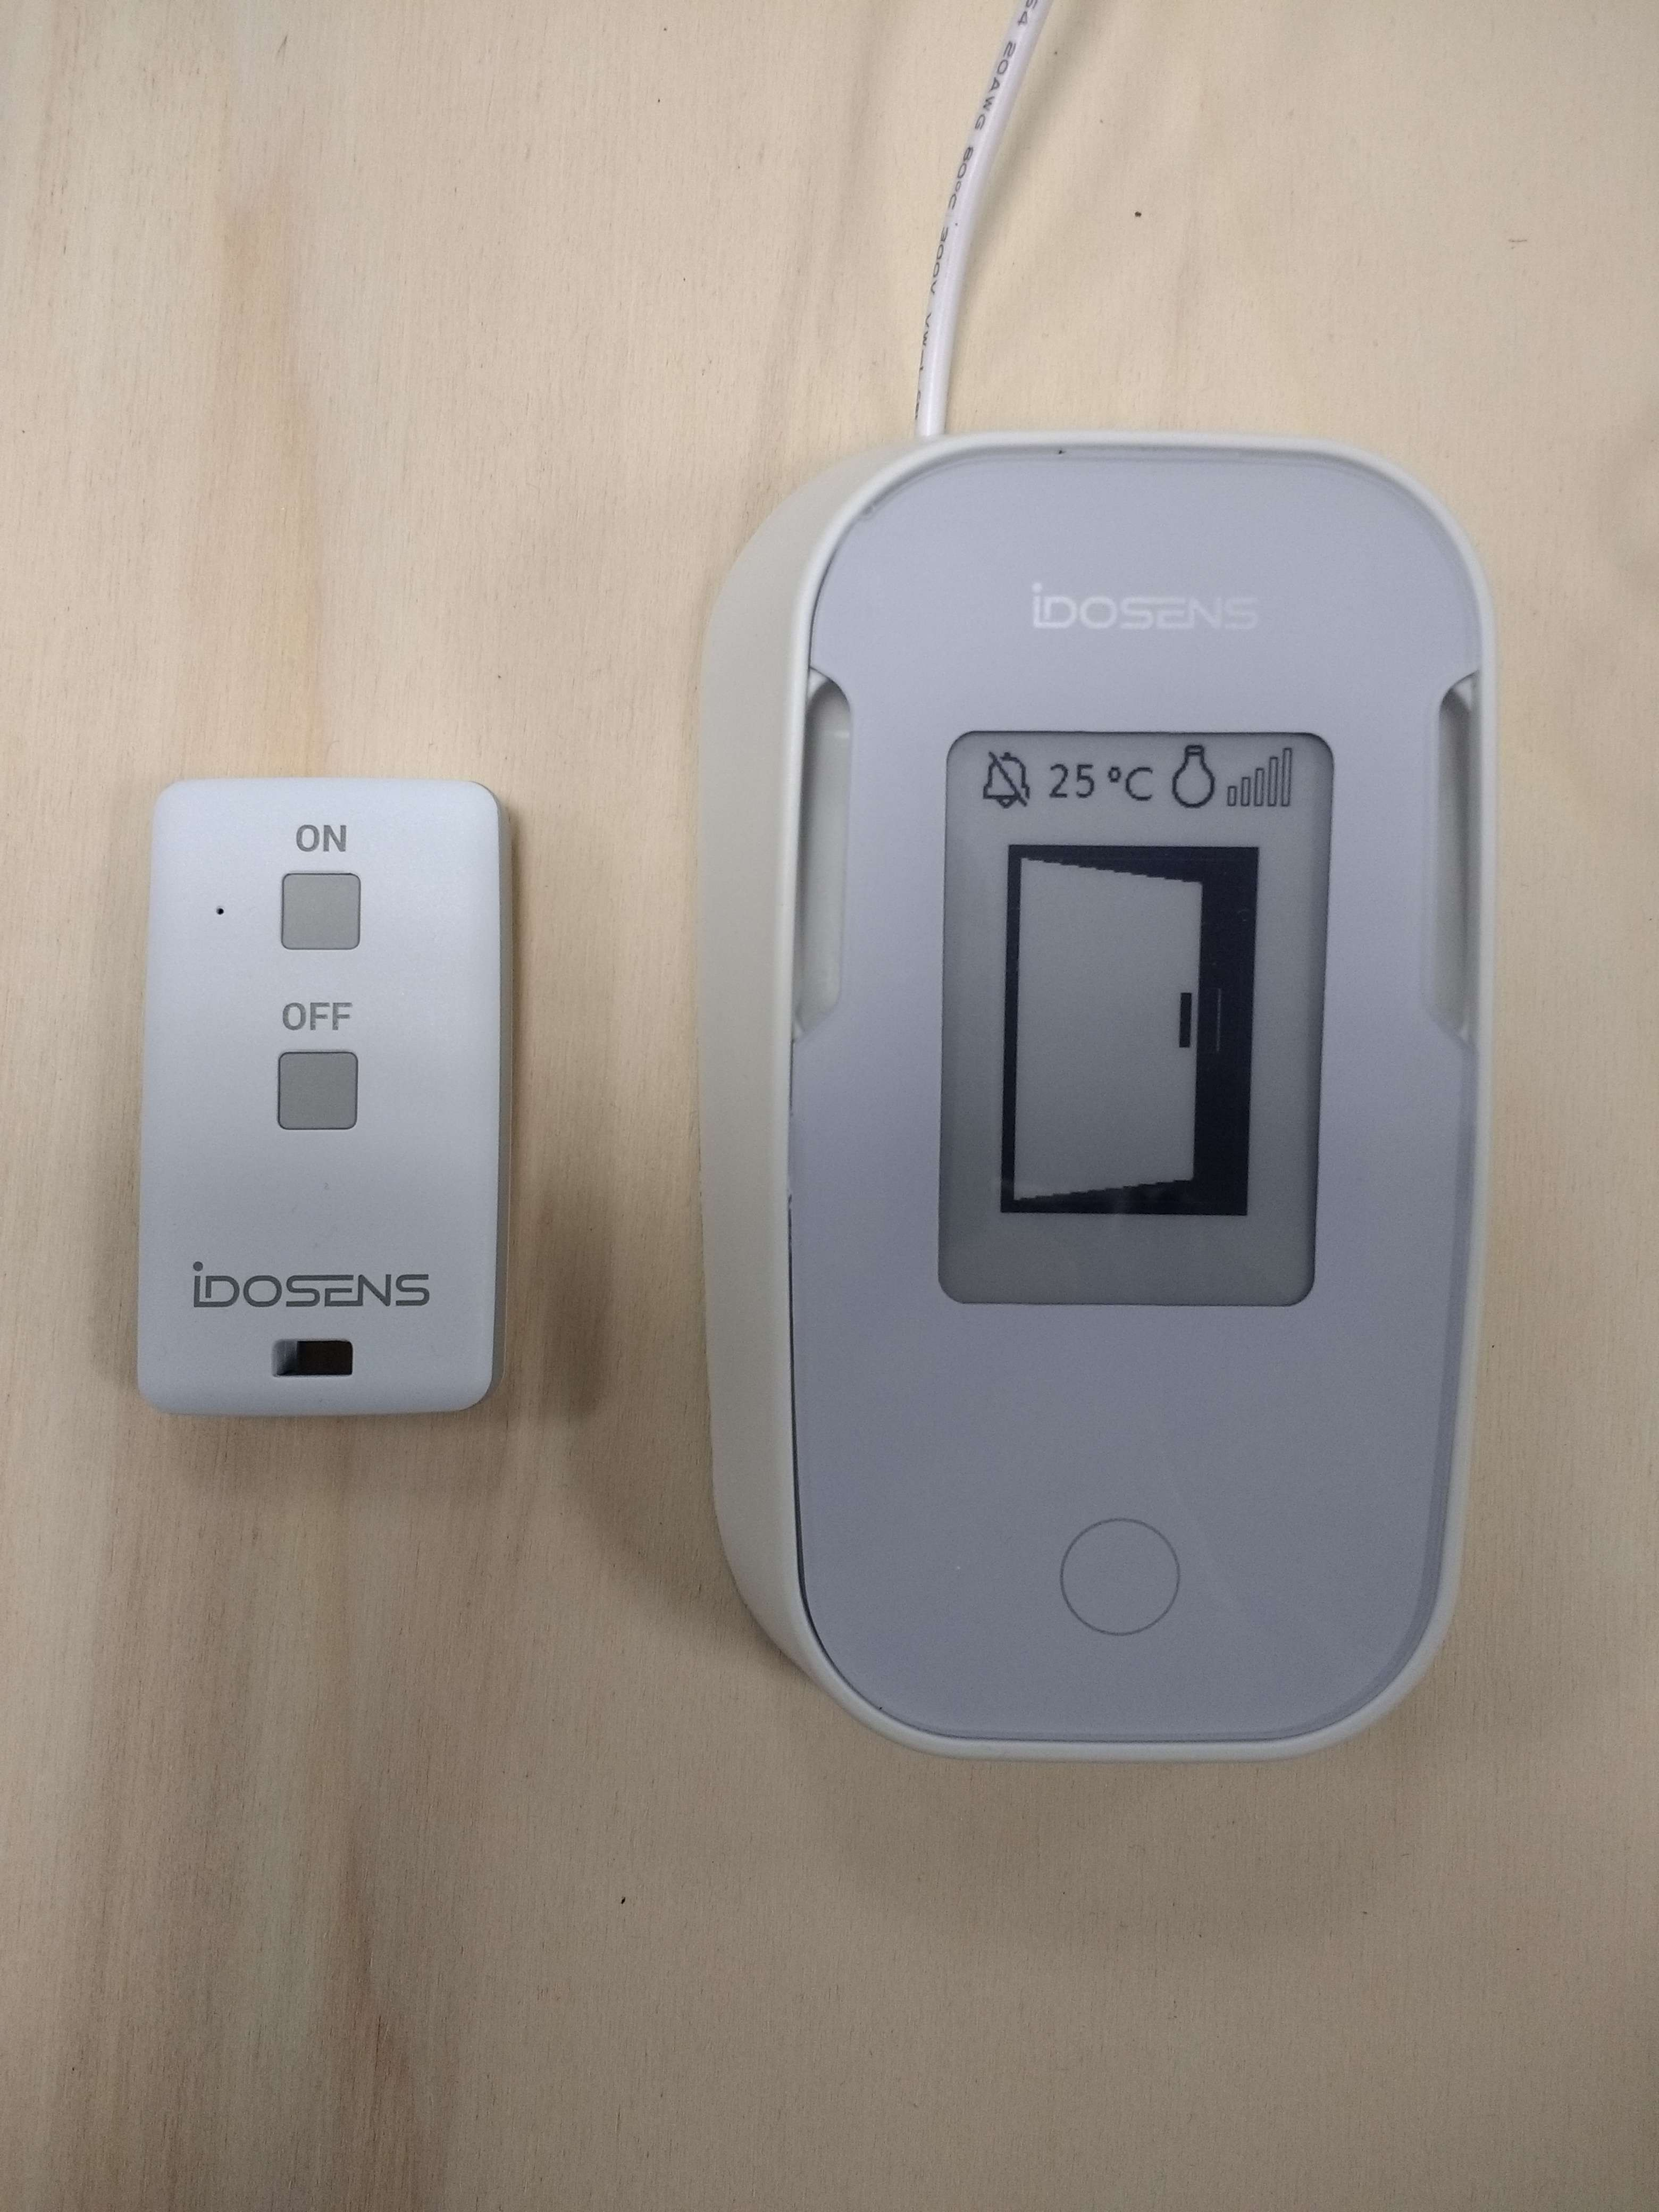
\includegraphics[keepaspectratio=true,scale=0.05]{produit_complet.jpg}
\label{visina8}
\end{center}\end{figure}

\begin{figure}[H]
  \centering
  \begin{minipage}[b]{0.45\textwidth}
    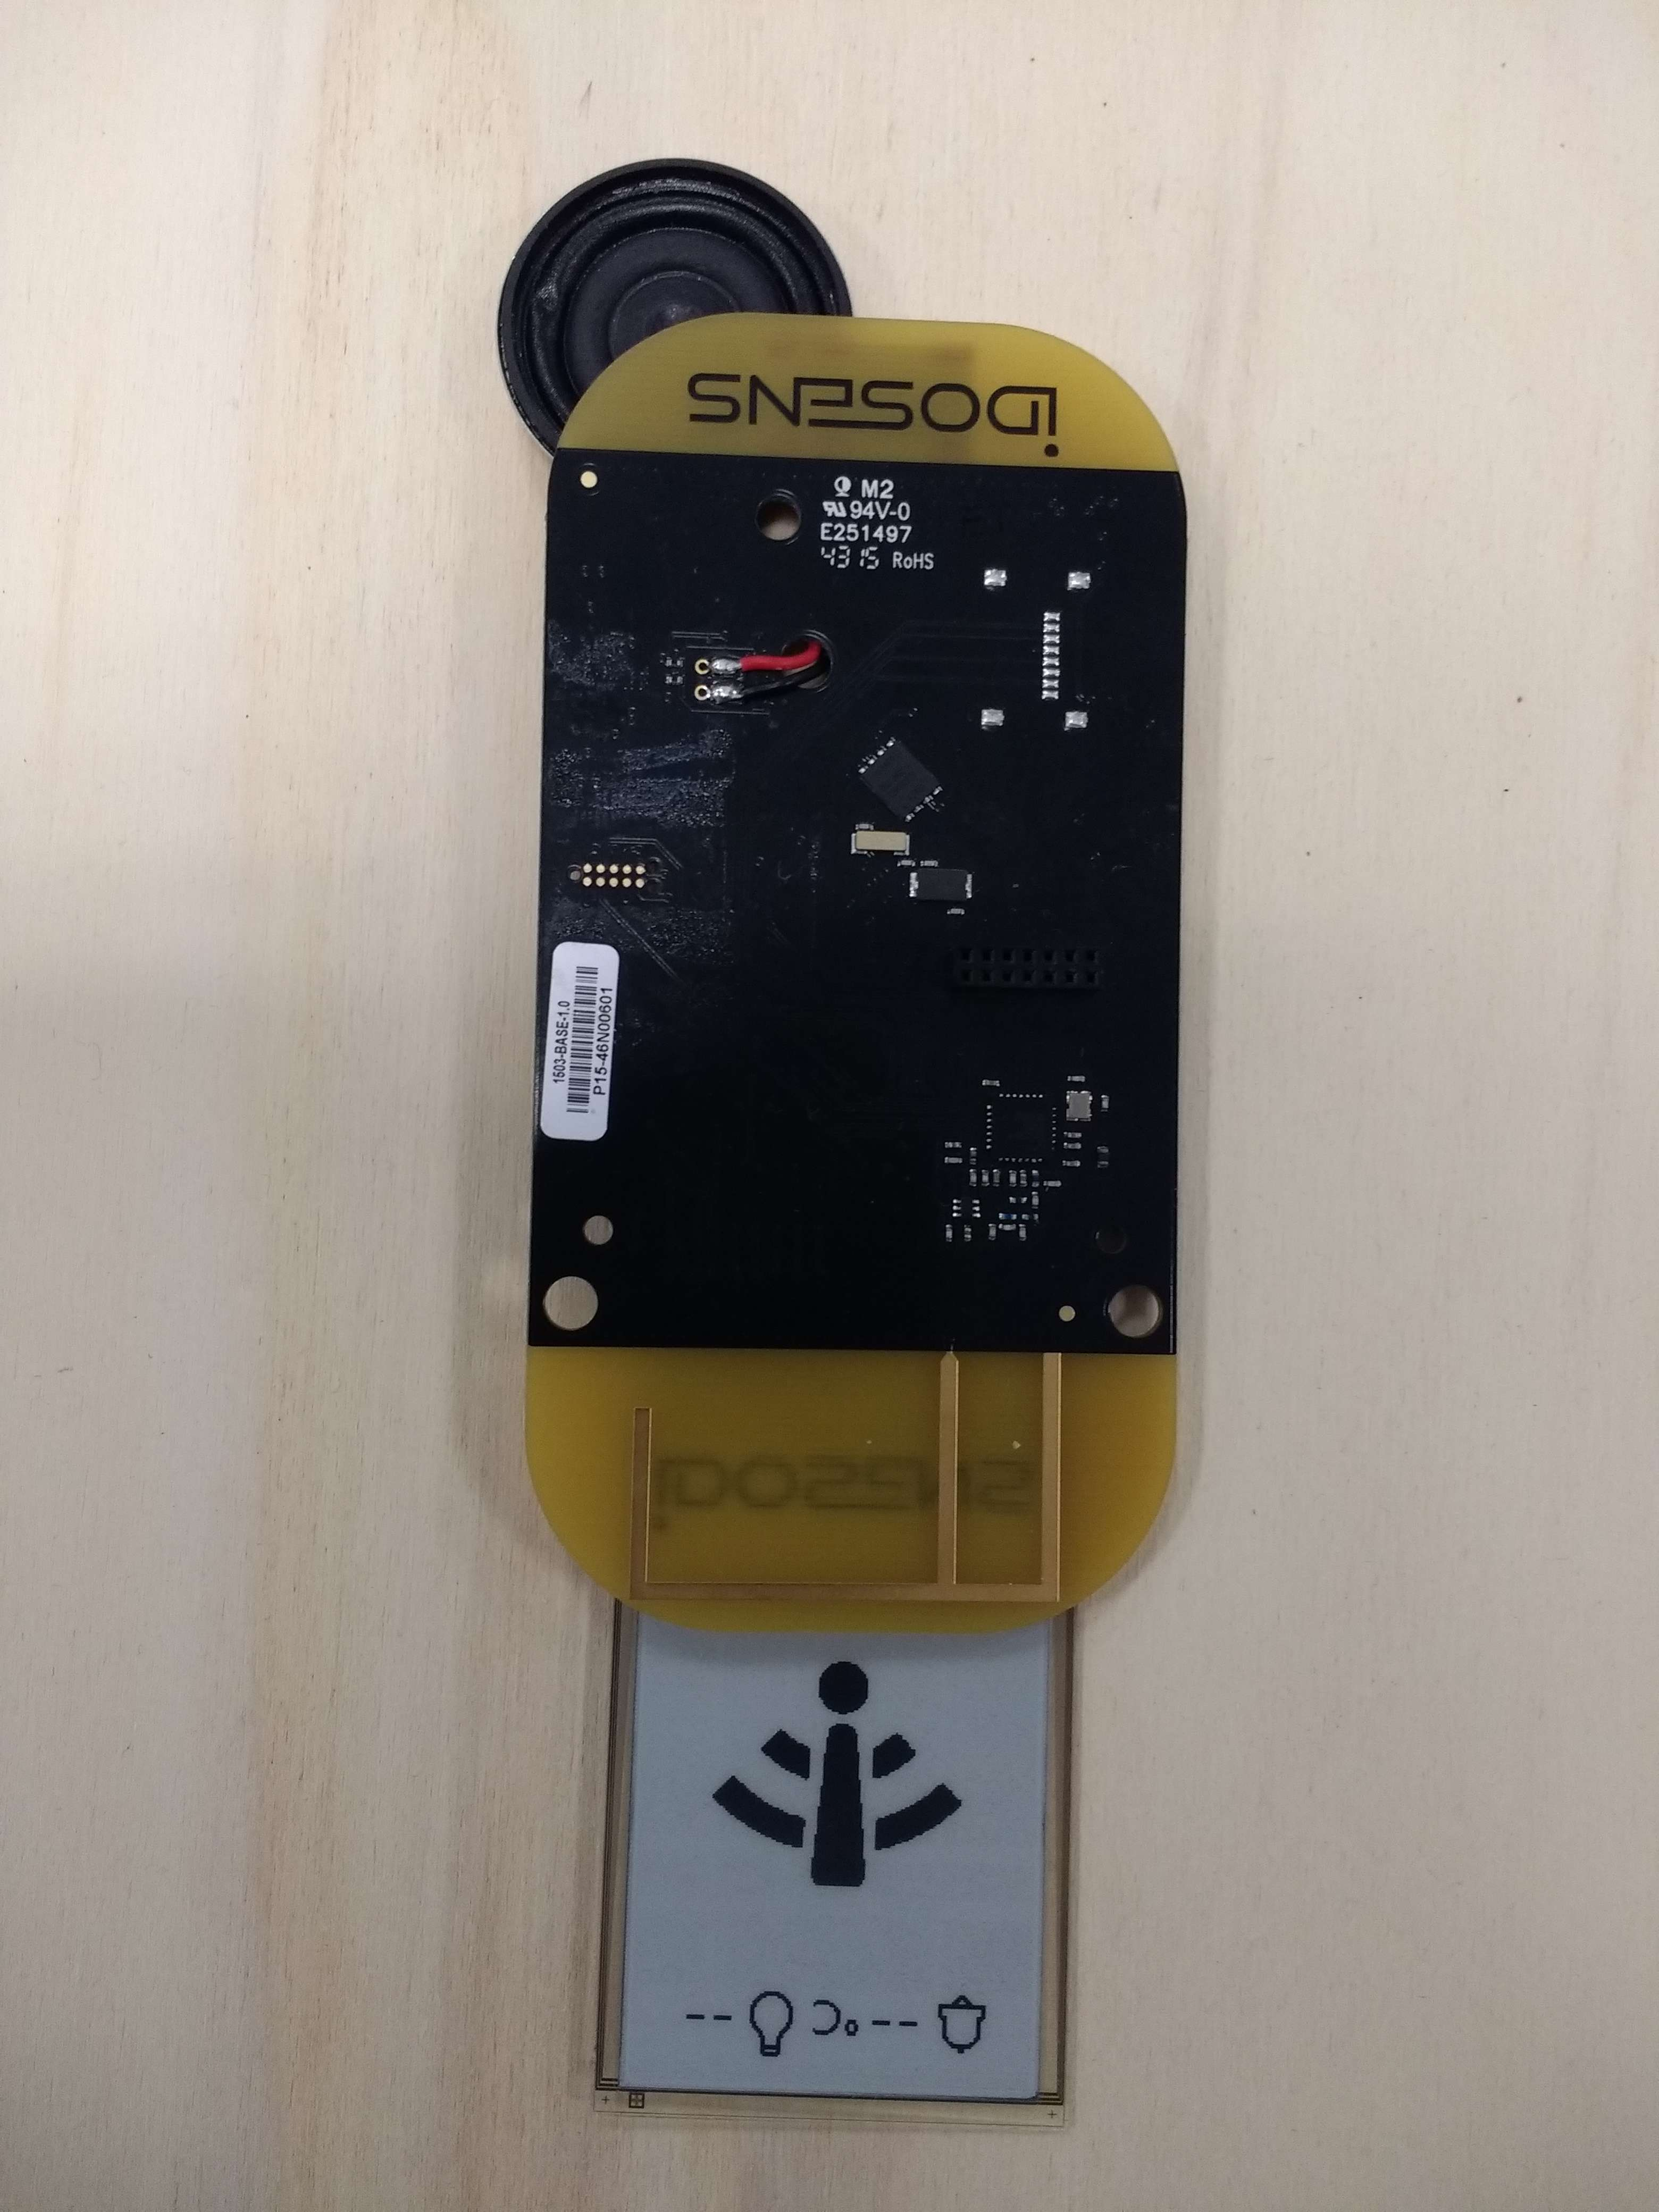
\includegraphics[width=\textwidth]{base_face.jpg}
    
  \end{minipage}
  \hfill
  \begin{minipage}[b]{0.45\textwidth}
    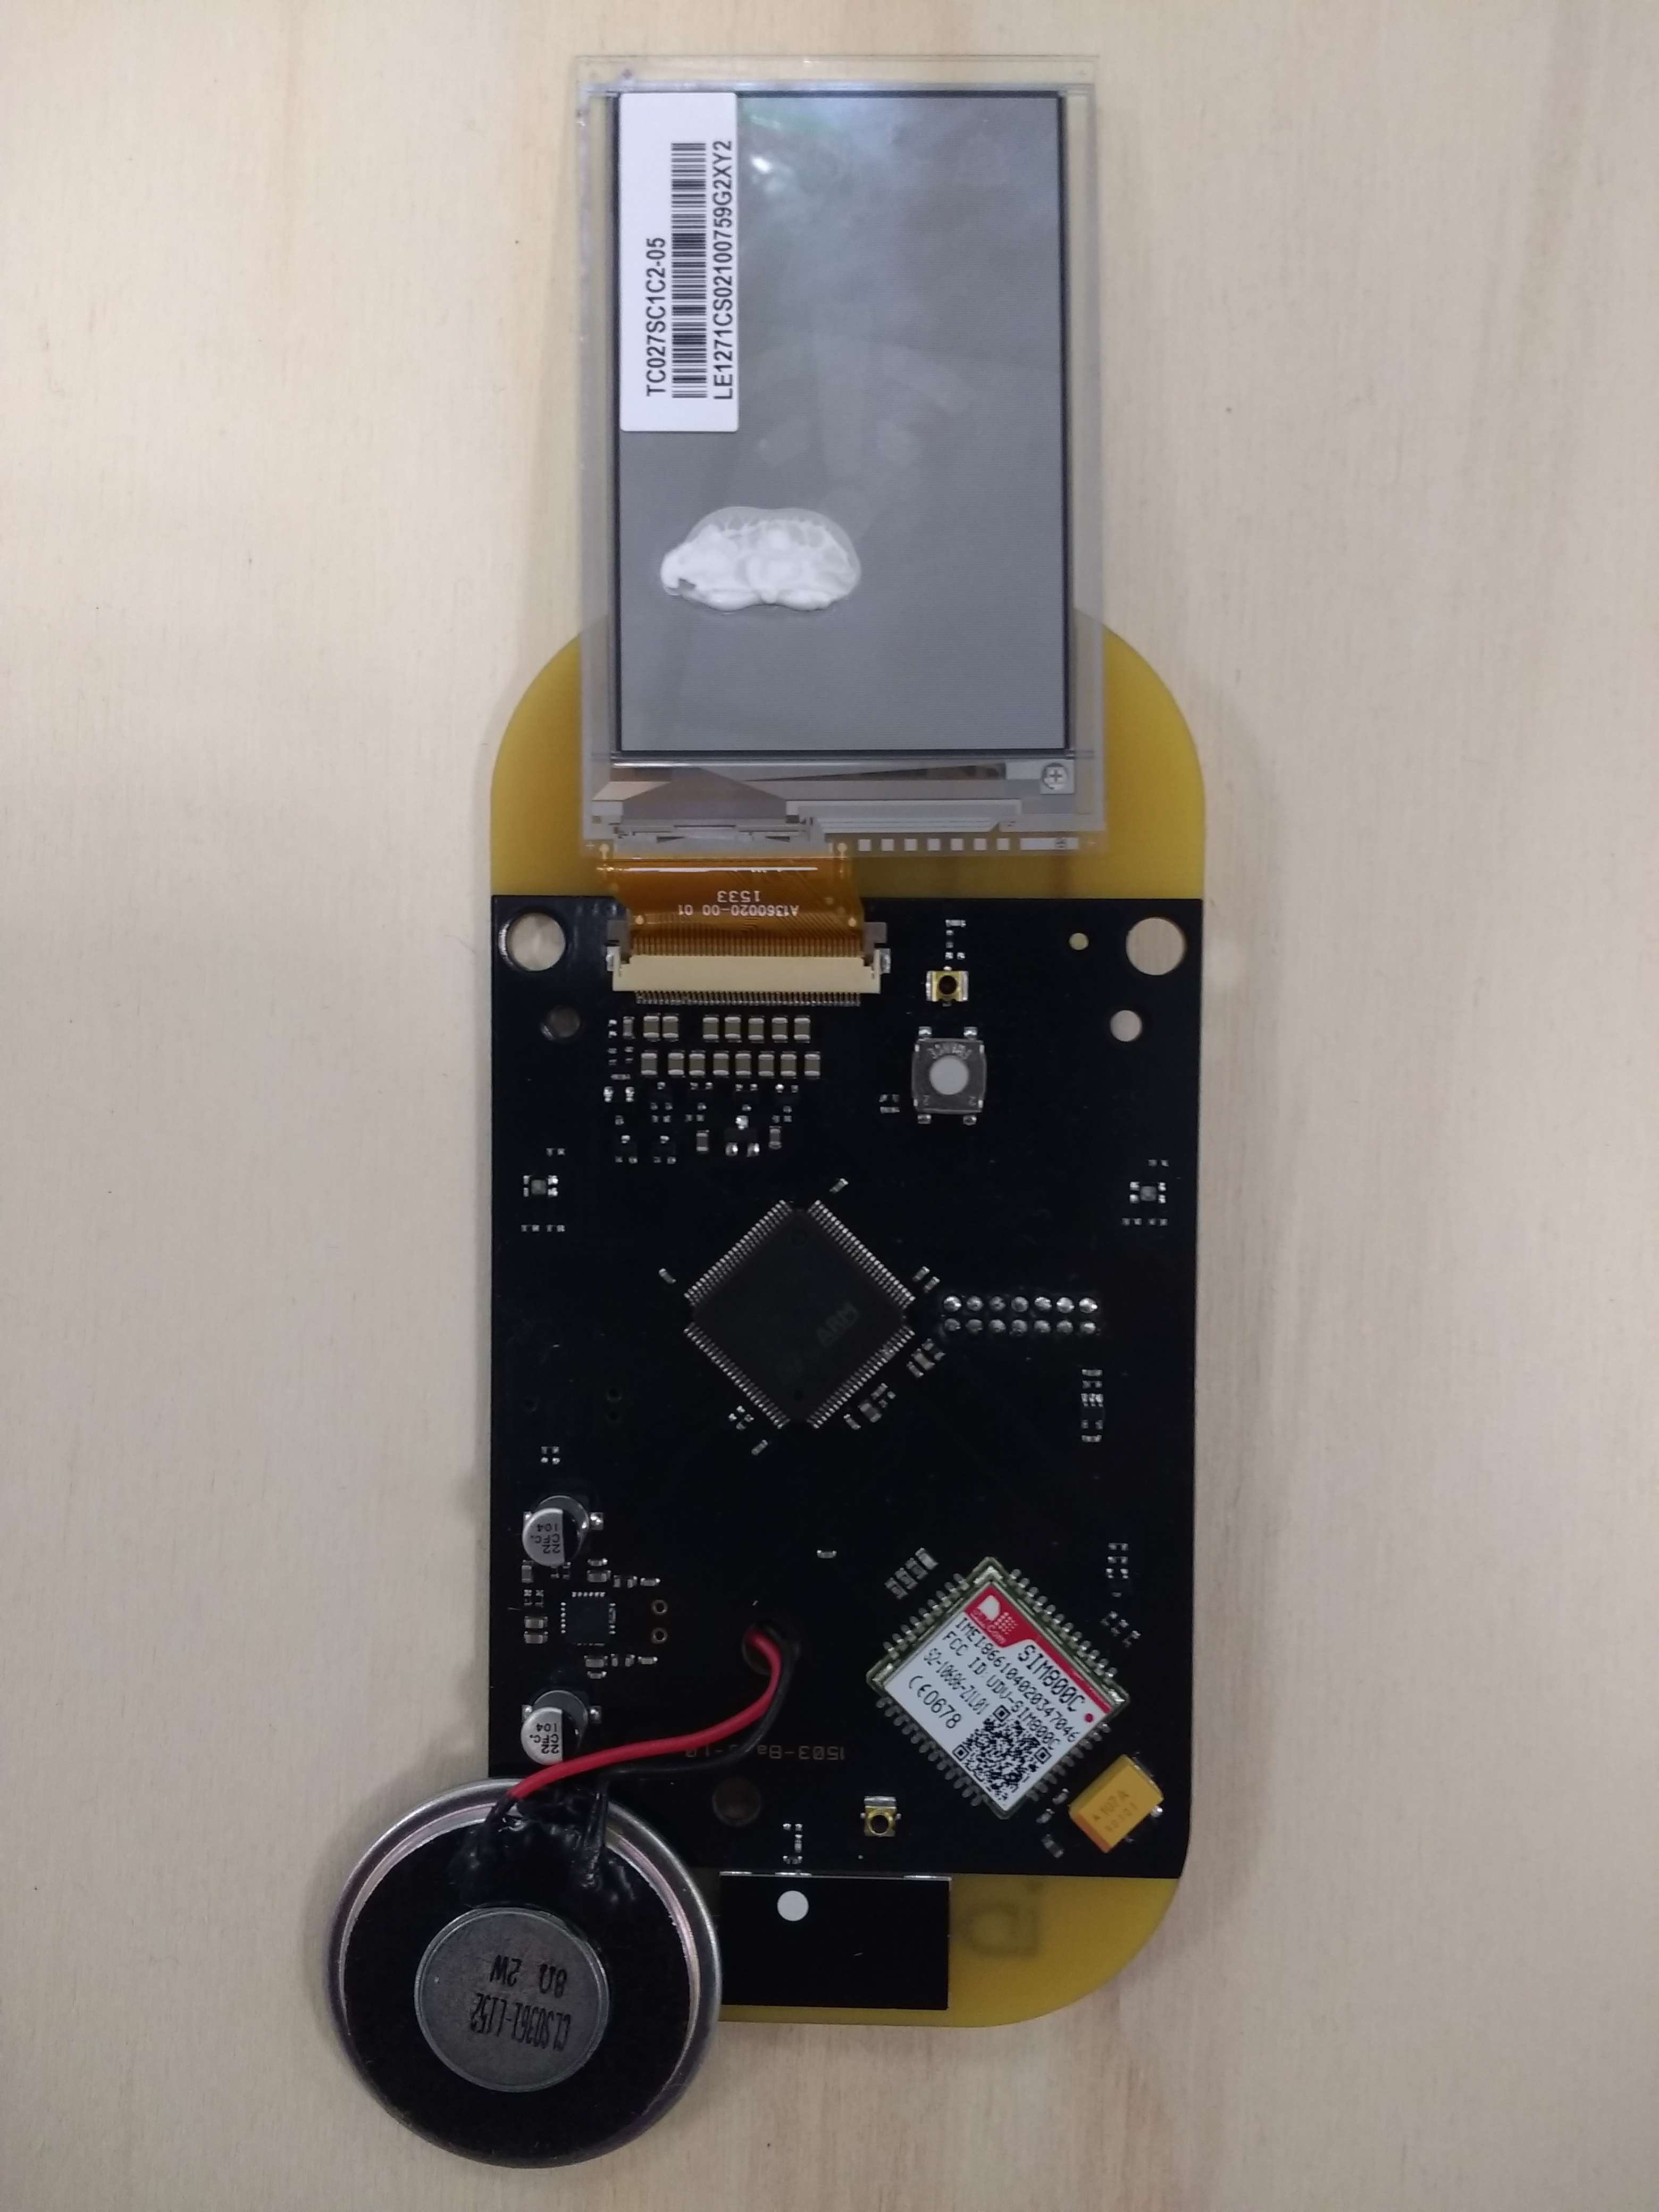
\includegraphics[width=\textwidth]{base_dos.jpg}
    
  \end{minipage}
\end{figure}


\begin{figure}[H]
  \centering
  \begin{minipage}[b]{0.45\textwidth}
    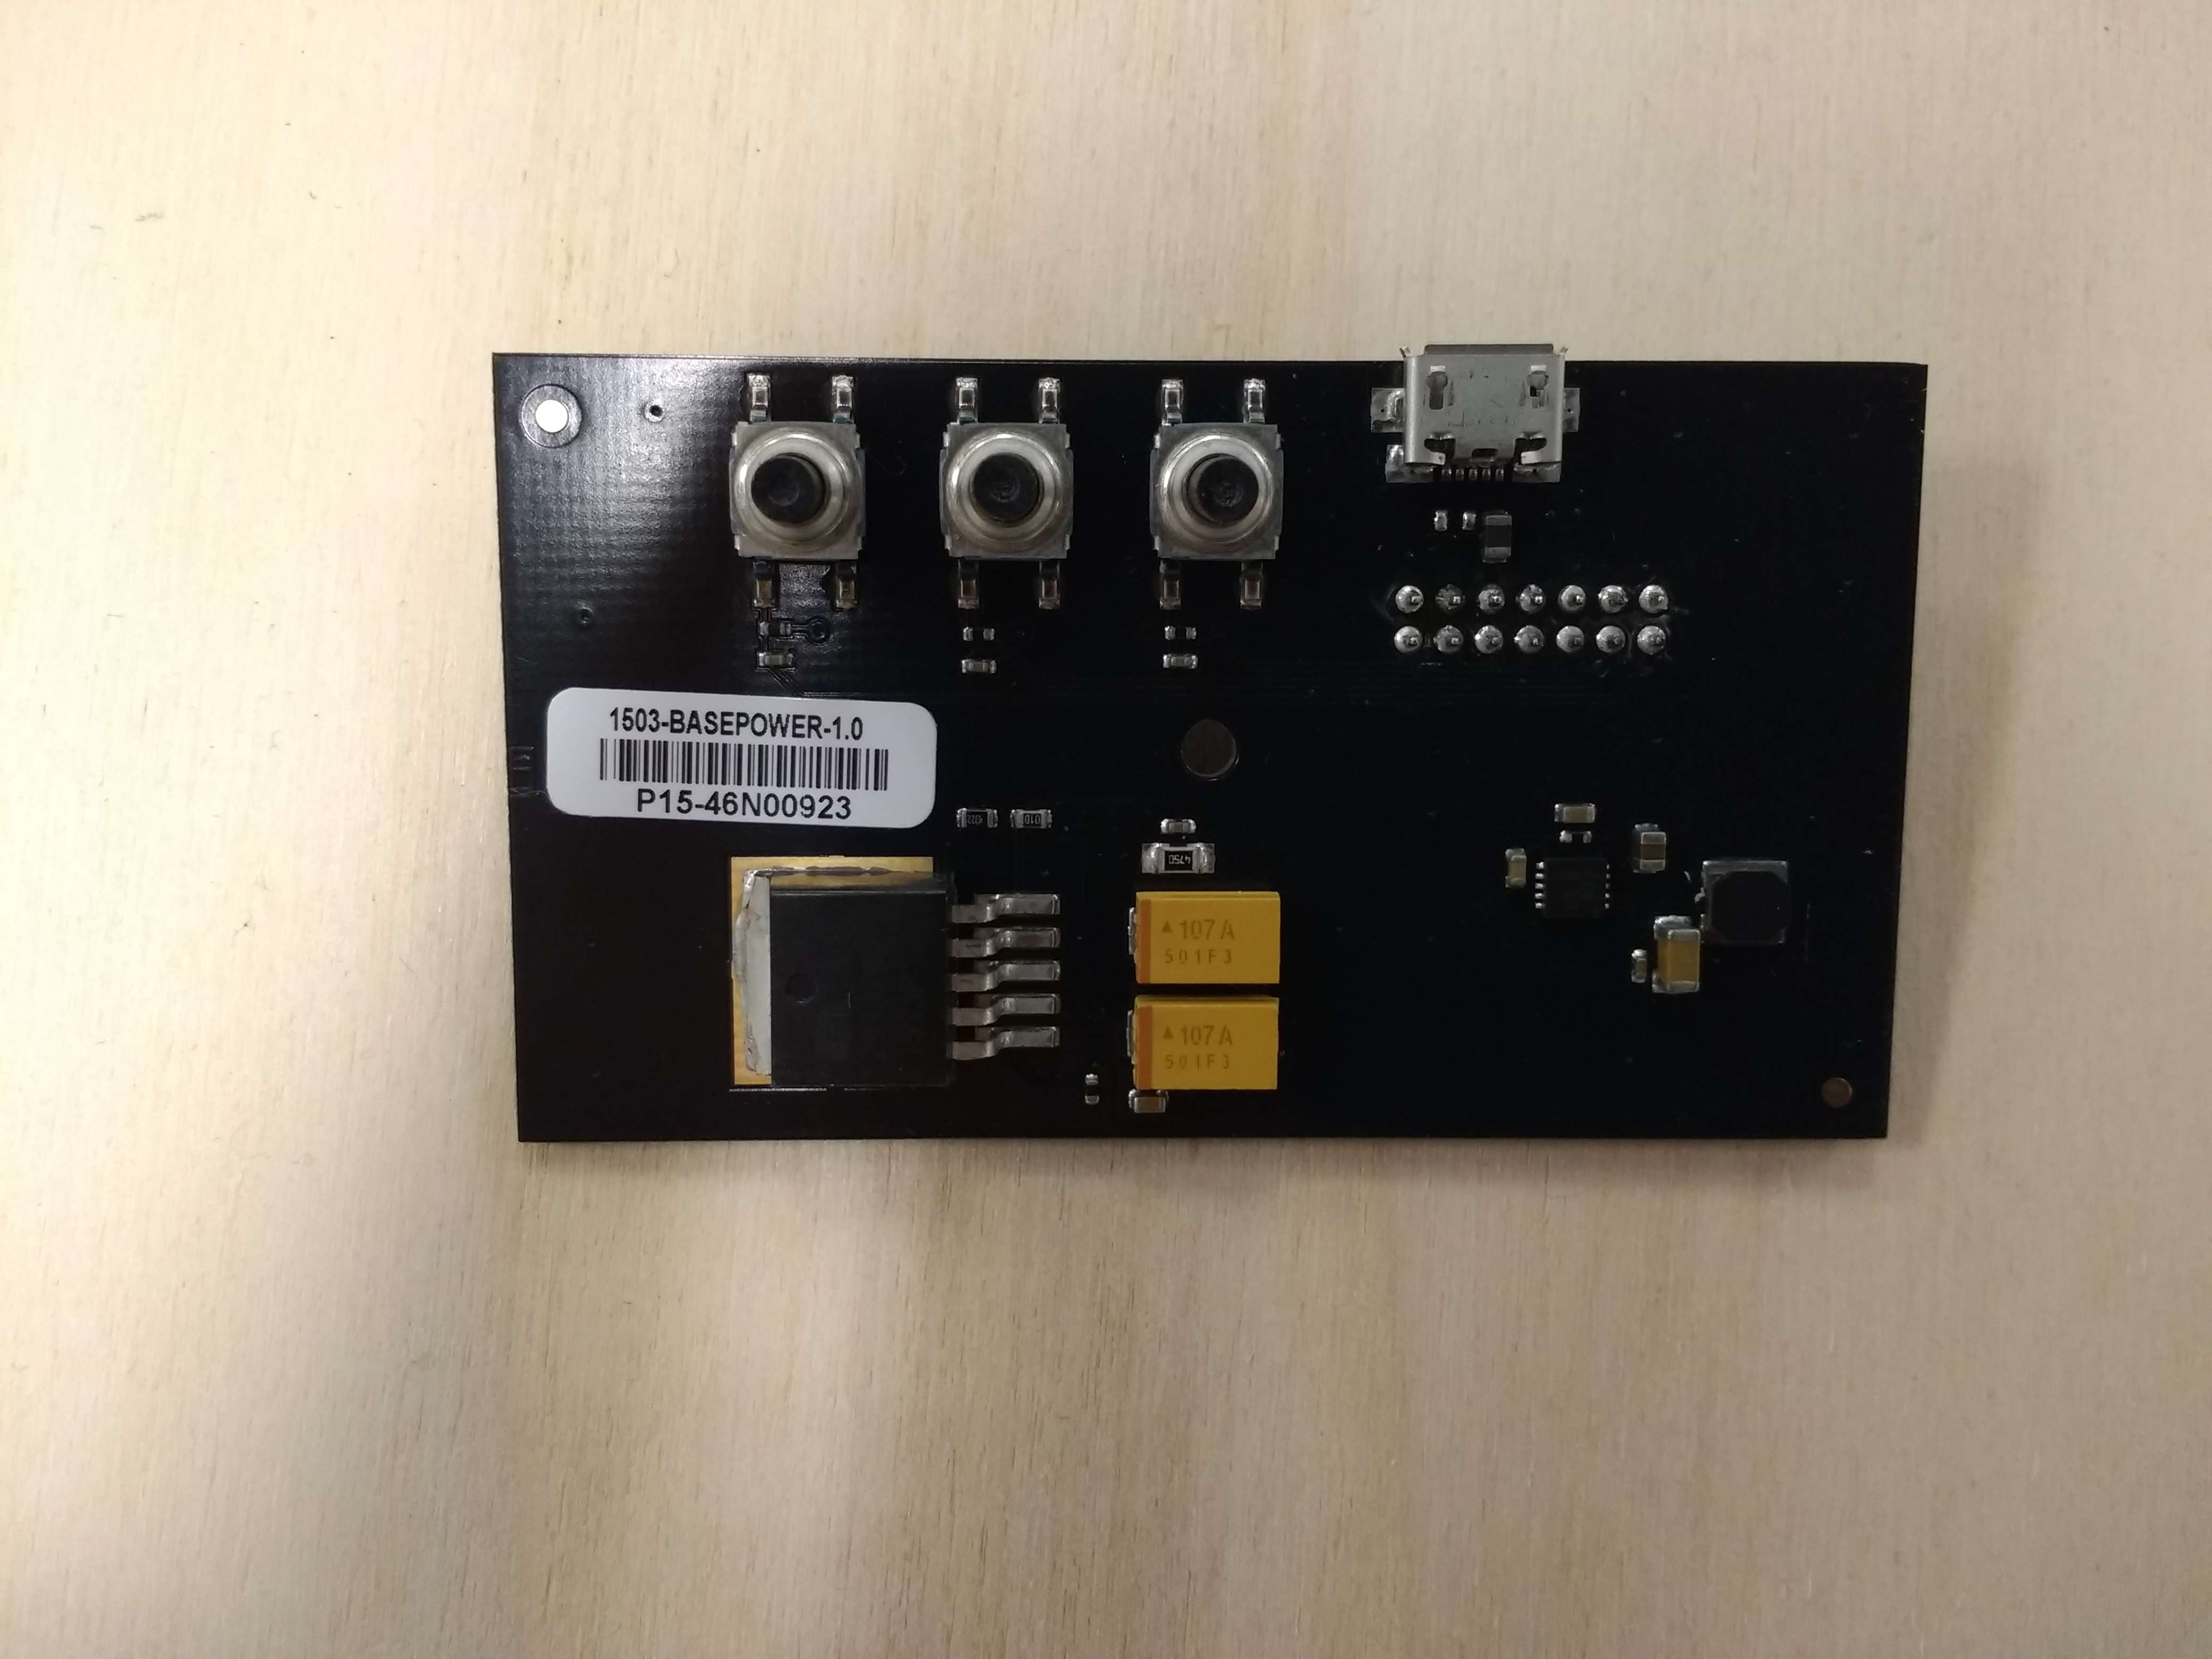
\includegraphics[width=\textwidth]{power_face.jpg}
    \caption{base power face}
  \end{minipage}
  \hfill
  \begin{minipage}[b]{0.45\textwidth}
    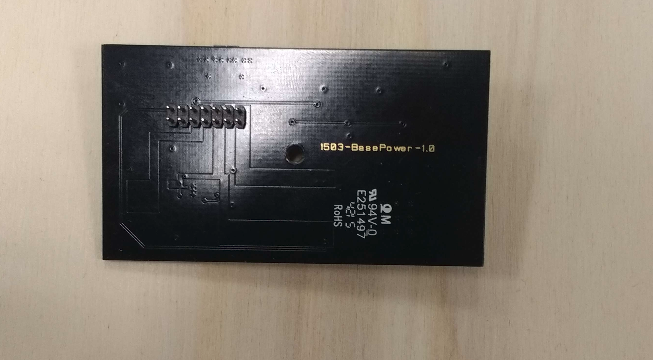
\includegraphics[width=\textwidth]{power_dos.png}
      \caption{base power dos}
  \end{minipage}
\end{figure}




\begin{figure}[H]
\begin{center}
\advance\leftskip-3cm
\advance\rightskip-3cm
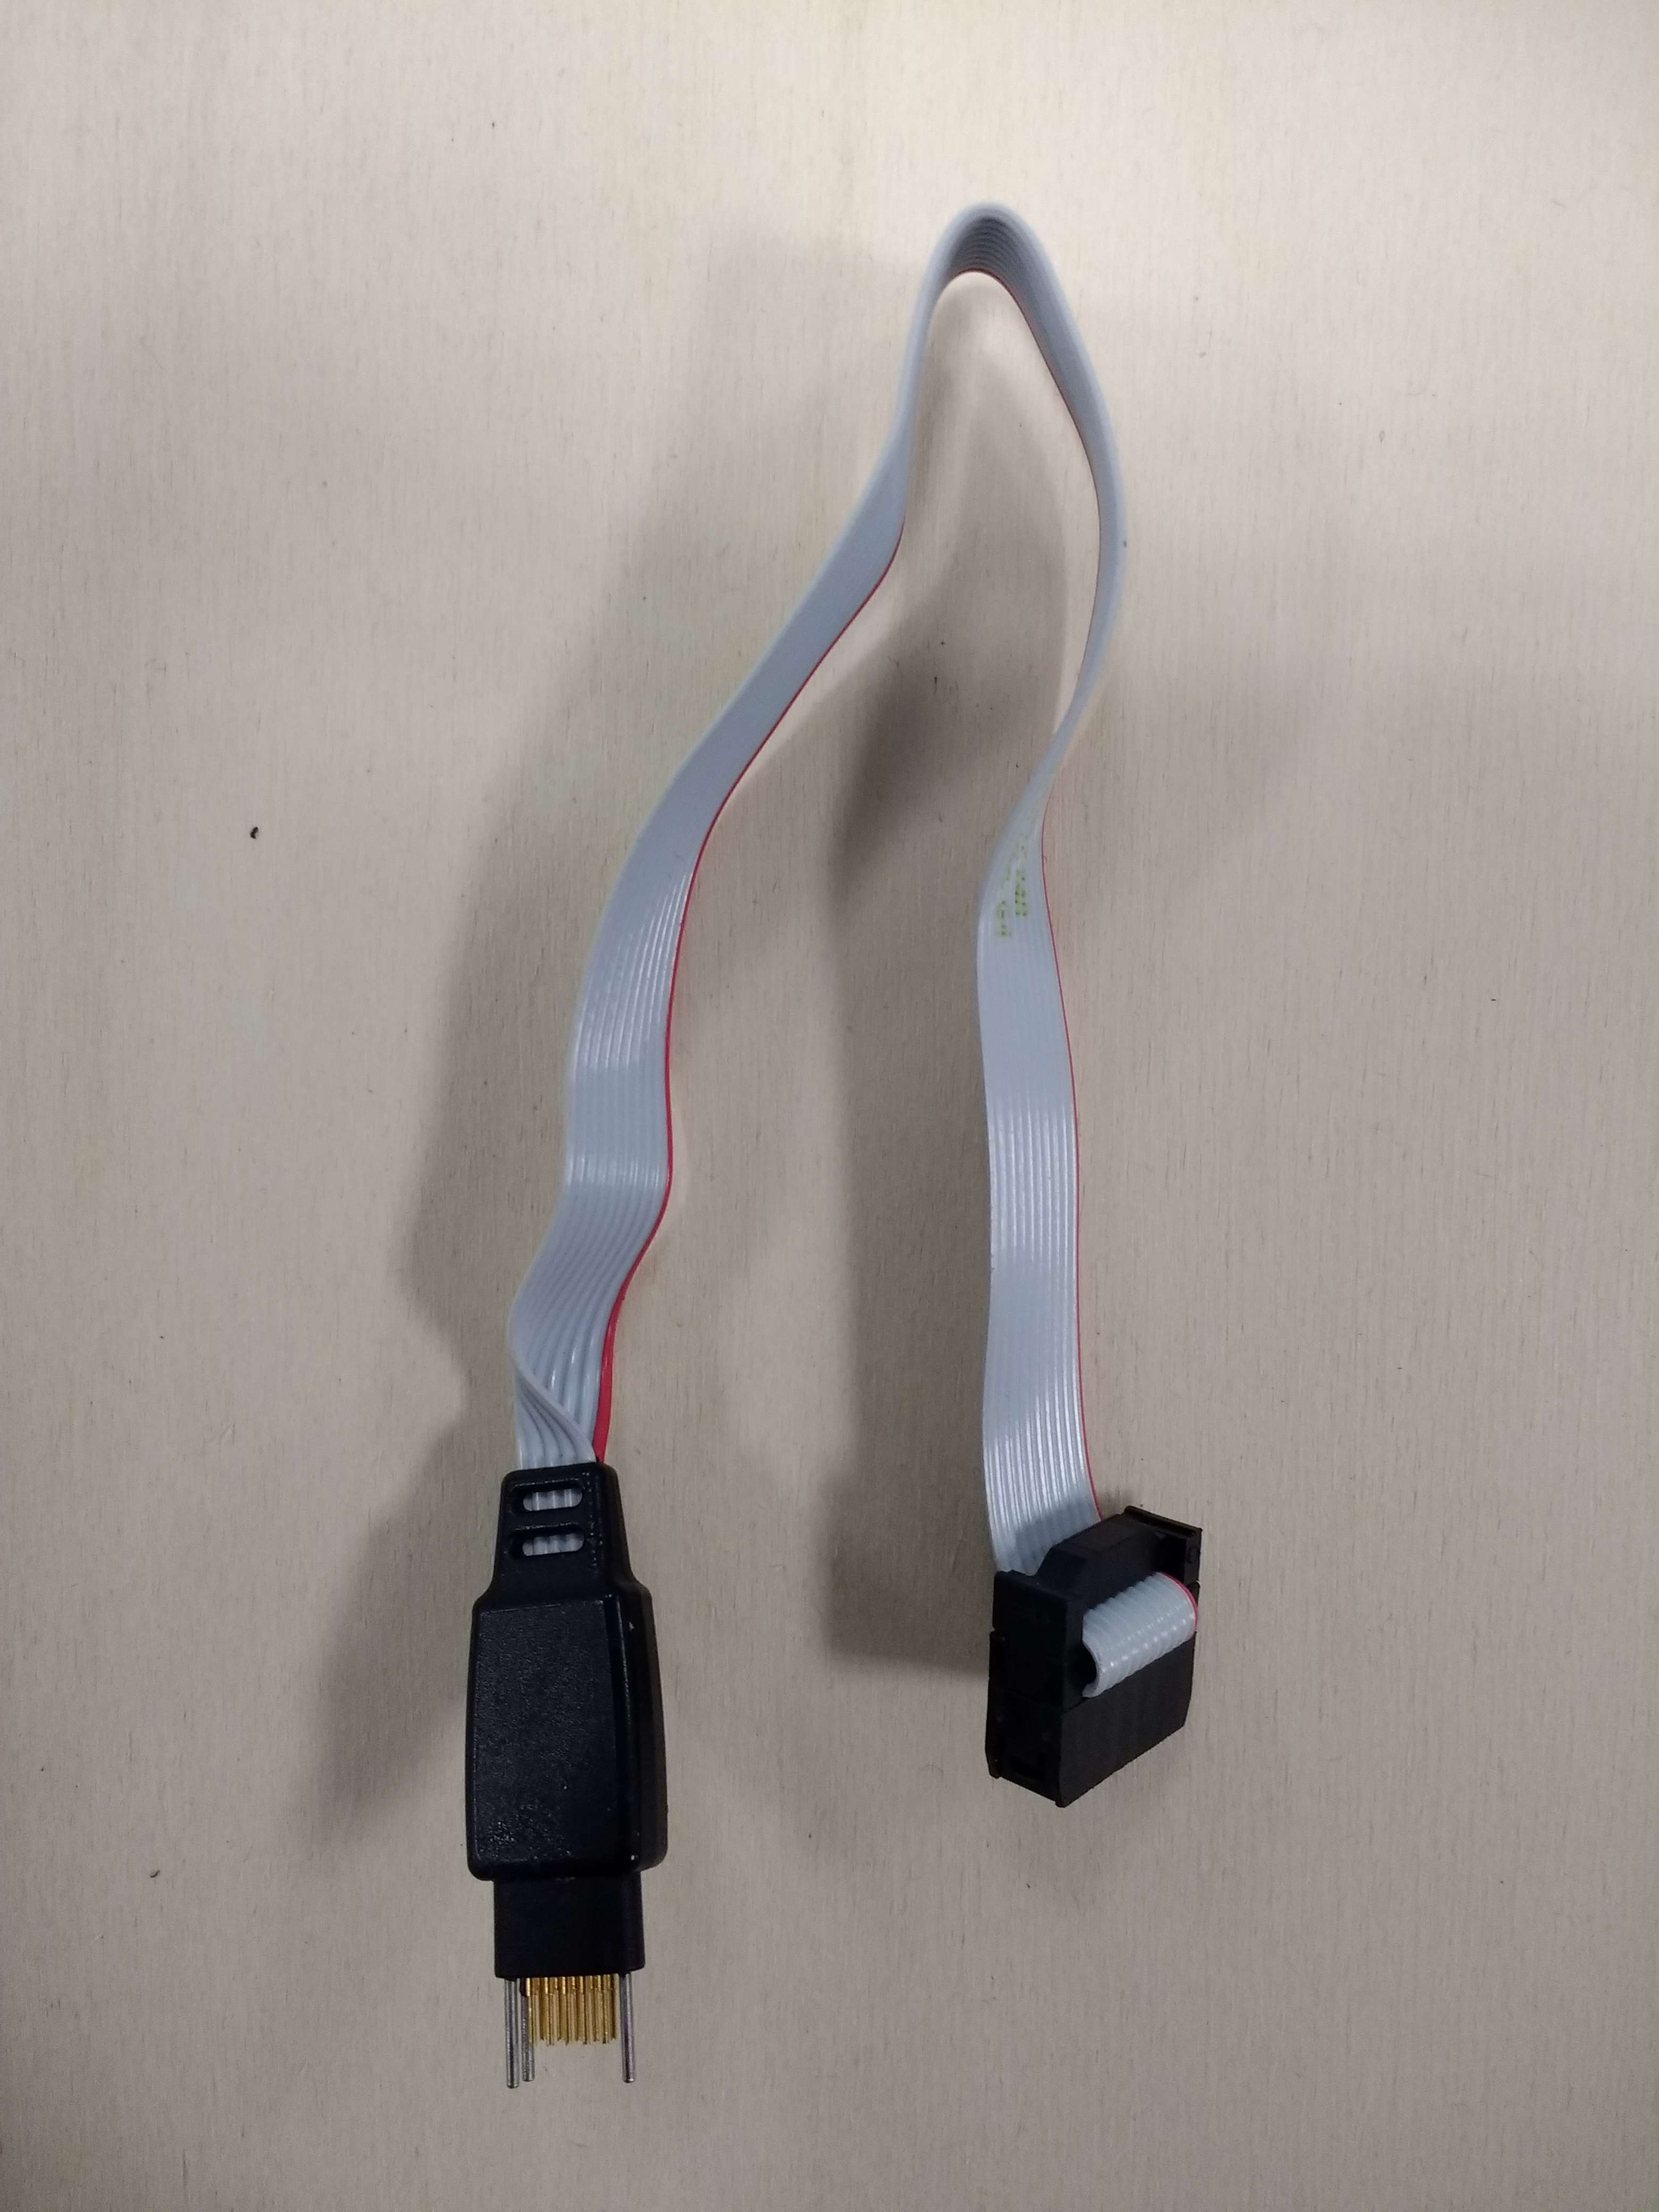
\includegraphics[keepaspectratio=true,scale=0.05]{tag_connect.jpg}
\caption{Tag connect}
\label{visina8}
\end{center}\end{figure}


\textbf{Microcontrôlleur : STM32F103VCT6}



\section{Générer le firmware}

\subsection{Logiciel à installer}
\subsubsection{STM32CubeIDE}
\begin{itemize}
    \item Se créer un compte et télécharger le logiciel à : \\
\url{https://www.st.com/en/development-tools/stm32cubeide.html}\\
Téléchargez .deb ou .linux

    \item Lancez l'installation :
    Dans le répertoire destination de l'extraction : 
    \begin{minted}{bash}
    
    chmod +x st-stm32cubeide_1.0.2_3566_20190716_0927_amd64.sh
    sudo ./st-stm32cubeide_1.0.2_3566_20190716_0927_amd64.sh

    \end{minted}
\end{itemize}

Pour lancer l'IDE allez dans le répertoire d'installation et double-cliquez sur stm32cubeide ou
\begin{minted}{bash}

./stm32cubeide&

\end{minted}

\subsection{Créer un projet}

Aller dans File, New, STM32 Project \\
Dans Target selecor, chercher STM32F103VC et choisir STM32F103VCTx.
\begin{figure}[H]
\begin{center}
\advance\leftskip-3cm
\advance\rightskip-3cm
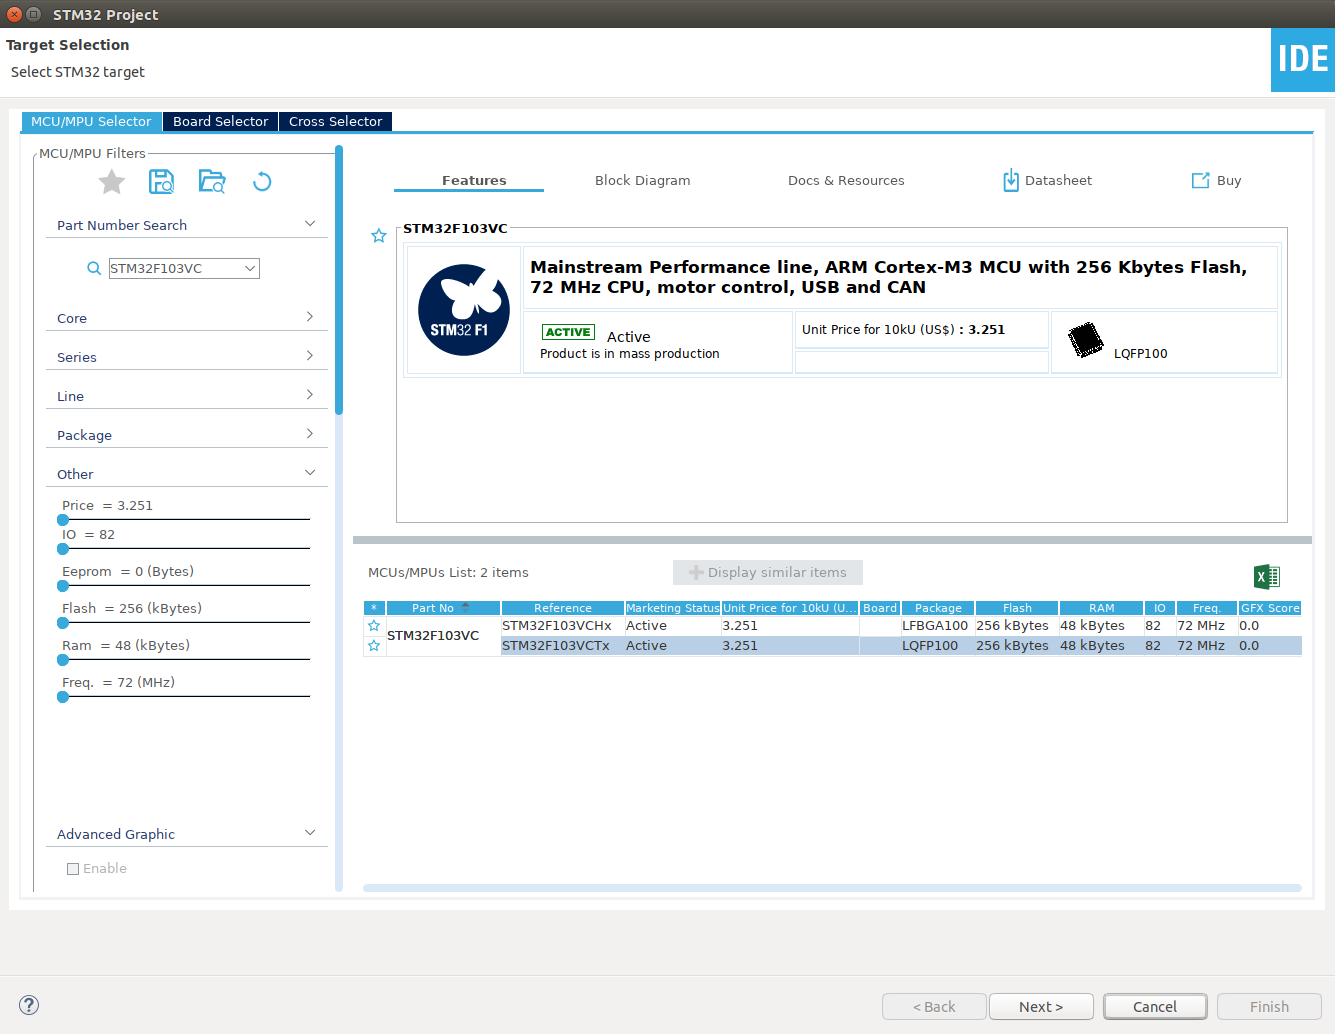
\includegraphics[keepaspectratio=true,scale=0.3]{target_selector.png}
\caption{Tag connect}
\label{visina8}
\end{center}\end{figure}

Créez le projet, puis choisissez "oui" pour la boîte de dialogue suivante à la fin de la création du projet :
\begin{figure}[H]
\begin{center}
\advance\leftskip-3cm
\advance\rightskip-3cm
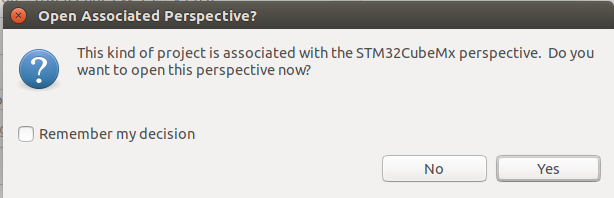
\includegraphics[keepaspectratio=true,scale=0.3]{end_projectcreation.png}
\caption{Tag connect}
\label{visina8}
\end{center}\end{figure}

STM32Cube IDE va lancer le "device configuration tool" qui permet d'activer l'UART et générer du code d'exemple pour celui-ci.

\begin{figure}[H]
\begin{center}
\advance\leftskip-3cm
\advance\rightskip-3cm
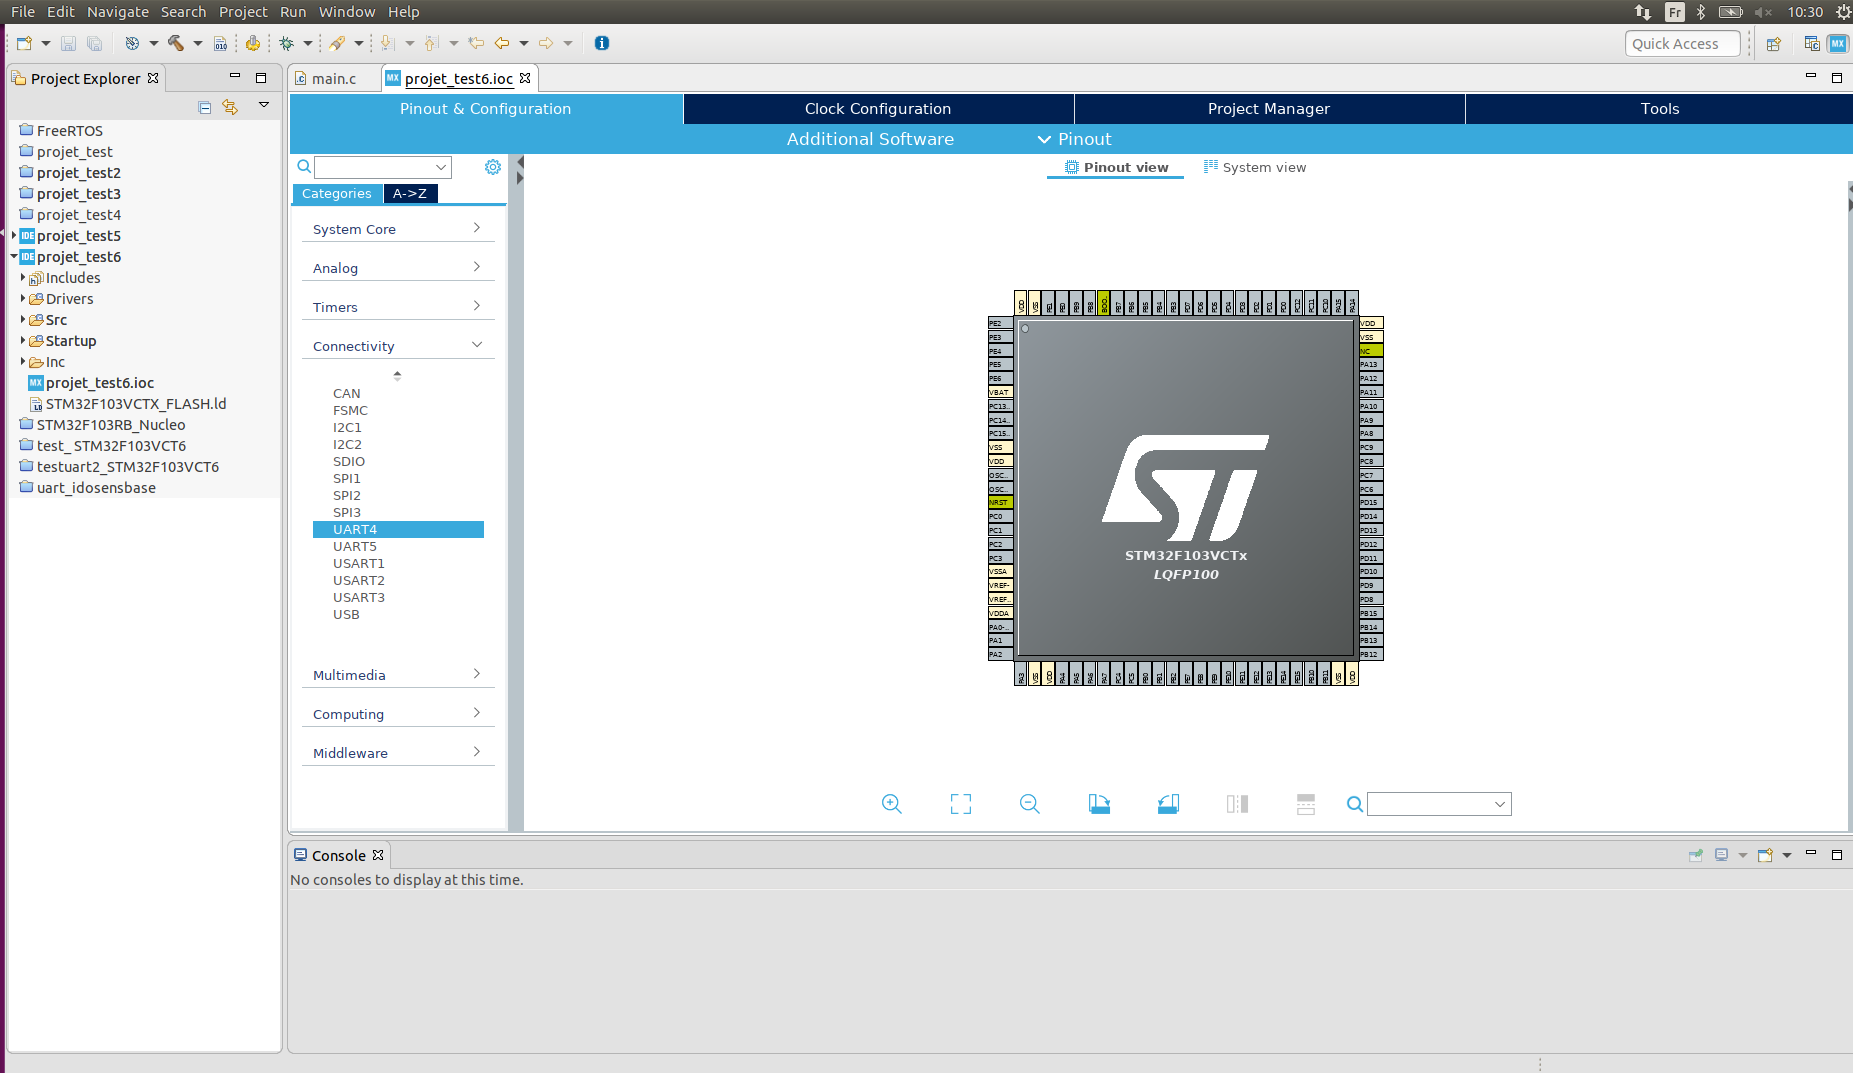
\includegraphics[keepaspectratio=true,scale=0.3]{configuration_tool.png}
\caption{Tag connect}
\label{visina8}
\end{center}\end{figure}

sélectionnez UART4 et choisir mode asynchronous

Sauvez le projet puis choissez de générer du code avec la boîte de dialogue suivante :

\begin{figure}[H]
\begin{center}
\advance\leftskip-3cm
\advance\rightskip-3cm
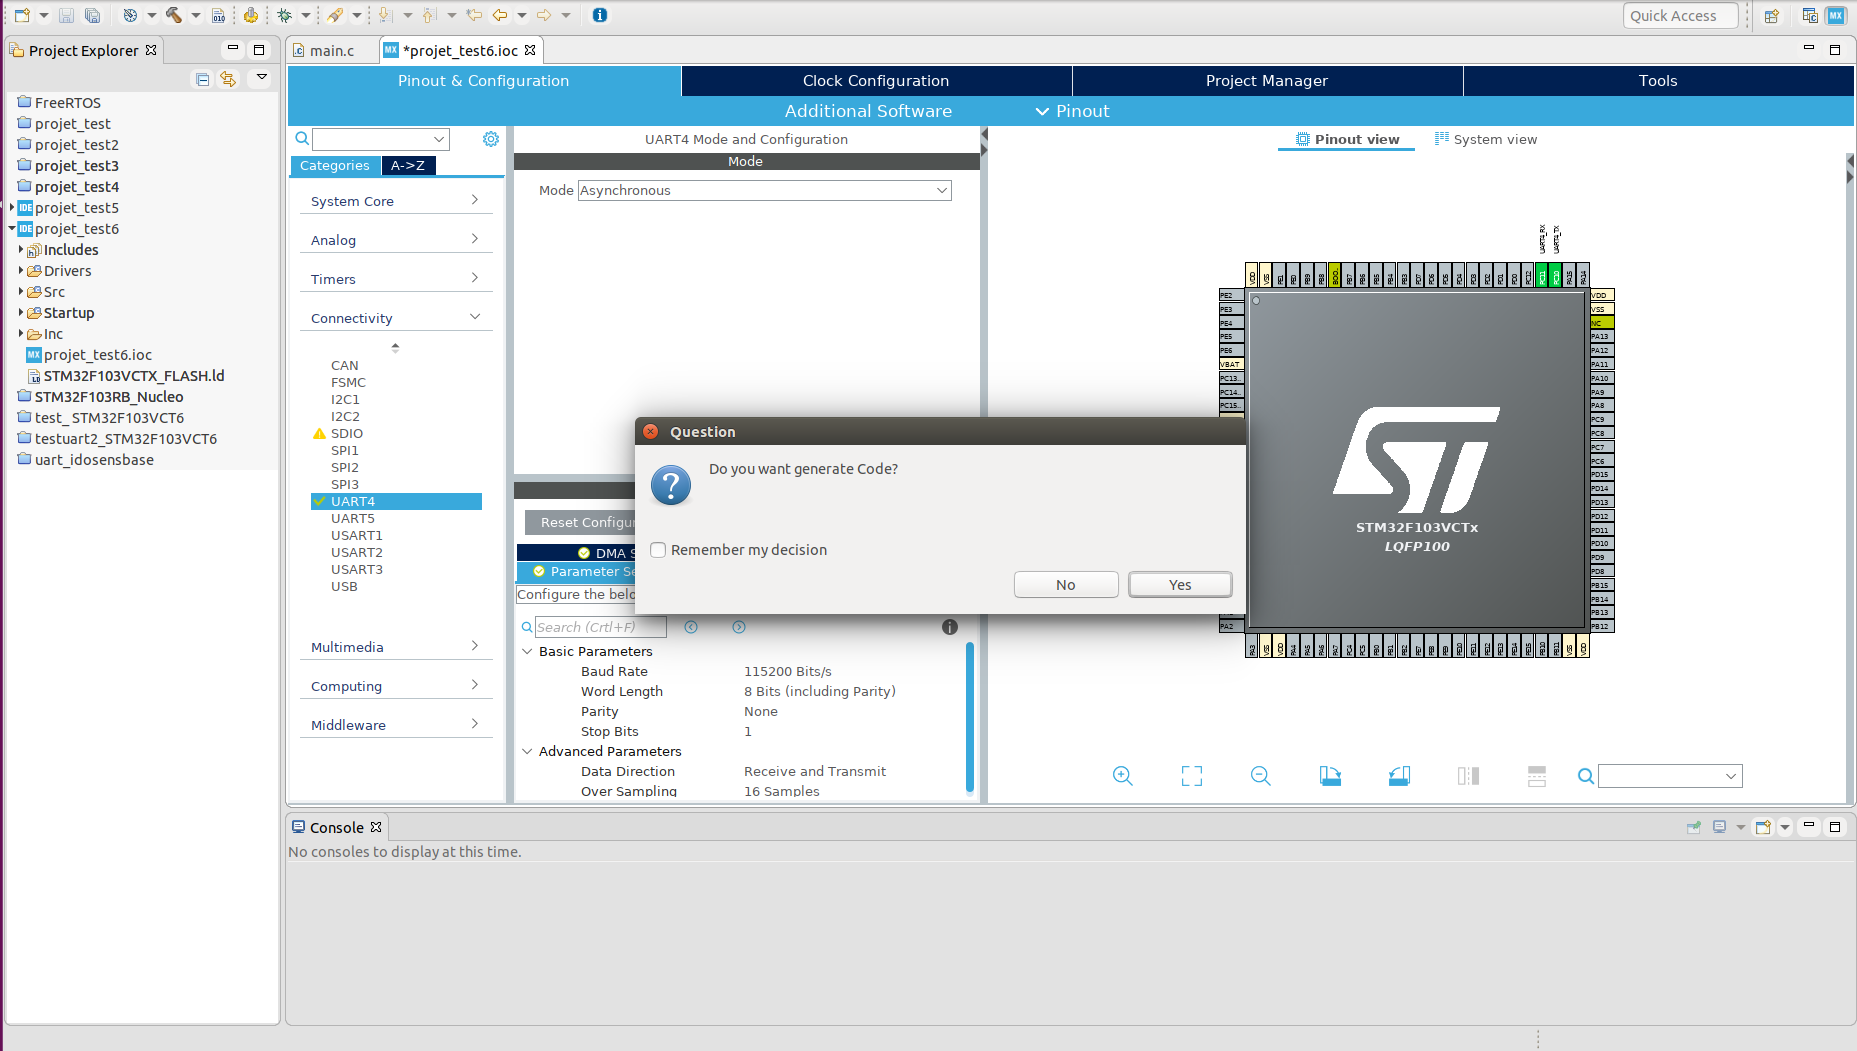
\includegraphics[keepaspectratio=true,scale=0.3]{do_you_wanttogeneratecode.png}
\caption{Tag connect}
\label{visina8}
\end{center}\end{figure}

Le code d'initialisation de l'UART est généré dans main.c

Copiez le main.c disponible à \url{https://github.com/GitClementtest/what_is_your_name_idosens} :


\subsection{Générer le .elf ou .bin}

pour générer le .bin ou le .elf, compilez le projet selon l'image :

\begin{figure}[H]
\begin{center}
\advance\leftskip-3cm
\advance\rightskip-3cm
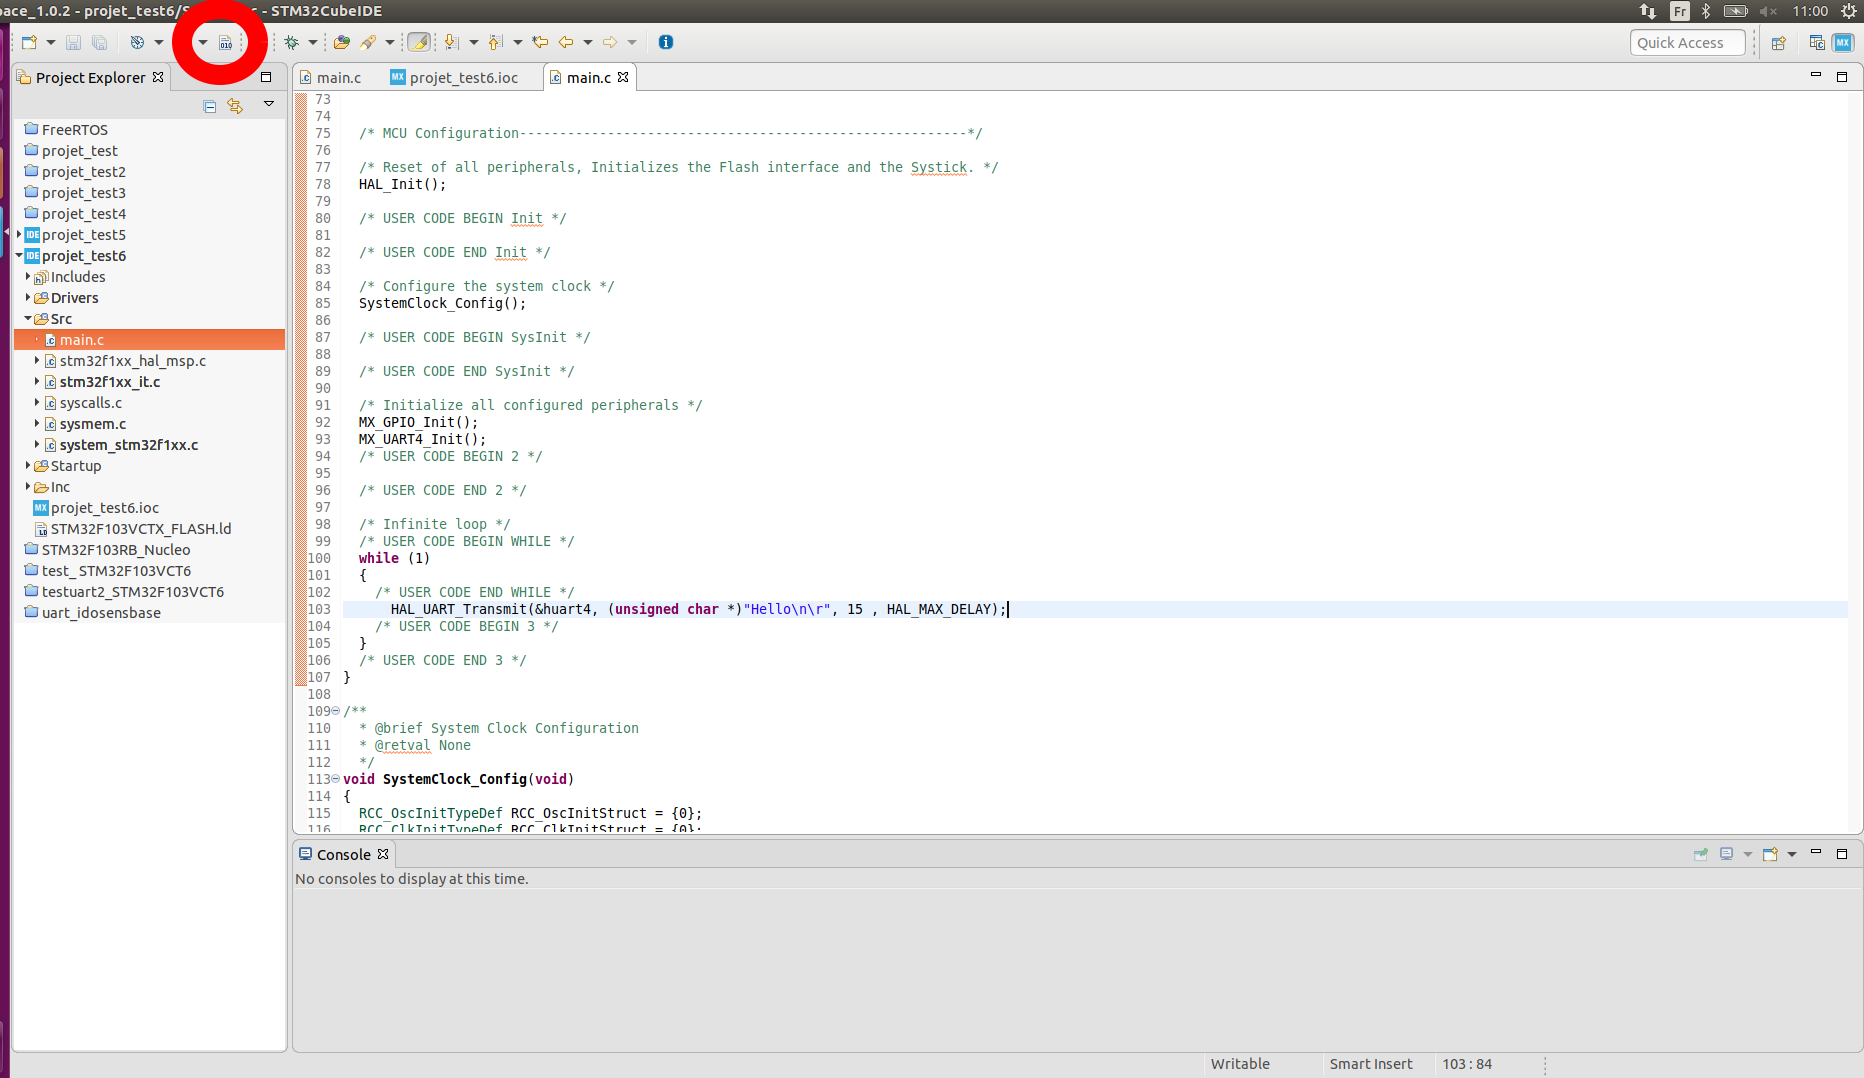
\includegraphics[keepaspectratio=true,scale=0.3]{build_all.png}
\caption{Tag connect}
\label{visina8}
\end{center}\end{figure}

Le fichier .elf se trouve dans le dossier Debug du projet.

\section{Flasher le code sur la carte}
\subsection{Logiciel à installer}
\subsubsection{STM32CubeProgrammer}
\textbf{Sur Ubuntu 16.04.6 LTS}

\begin{itemize}
   



 \item Avant de lancer l'installer :
\begin{minted}{bash}

sudo apt-get install openjfx

\end{minted}

 \item Se créer un compte et télécharger le logiciel à : \\

\url{https://www.st.com/en/development-tools/stm32cubeprog.html}


Lancez l'installer .linux 
\begin{minted}{bash}

./path_of_file.linux

\end{minted}



\item Téléchargez STSW-LINK007 à : \\ 
\url{https://www.st.com/en/development-tools/stsw-link007.html}


\item Ajouter des règles dans /etc/udev/rules.d

\begin{minted}{bash}

cd /extraction_path/stsw-link007/AllPlatforms/StlinkRulesFilesForLinux

sudo cp *.* /etc/udev/rules.d

sudo udevadm control --reload-rules #ou rebooter le PC


\end{minted}

\end{itemize}

\subsection{Si nécessaire}

\begin{itemize}
    



\item Installer libusb

\begin{minted}{bash}


sudo apt-get install libusb-1.0


\end{minted}

\item  upgrader STlink :

\begin{figure}[H]
\begin{center}
\advance\leftskip-3cm
\advance\rightskip-3cm
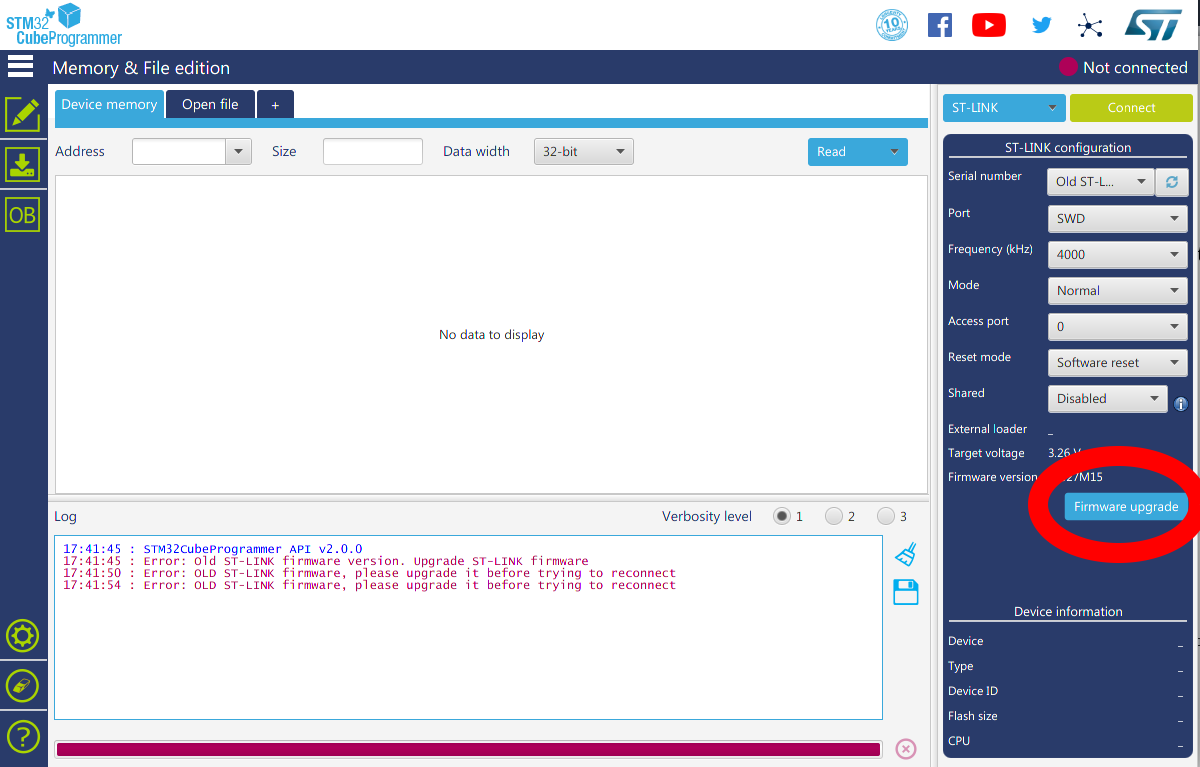
\includegraphics[keepaspectratio=true,scale=0.3]{stlink_upgrade.png}
\label{visina8}
\end{center}\end{figure}



\end{itemize}


\subsection{Connecter le produit idosens au PC}

\subsubsection{Connecter le Tag-connect à un débuggeur nucleo}
Détachez un débuguer d'une carte nucleo :

\begin{figure}[H]
\begin{center}
\advance\leftskip-3cm
\advance\rightskip-3cm
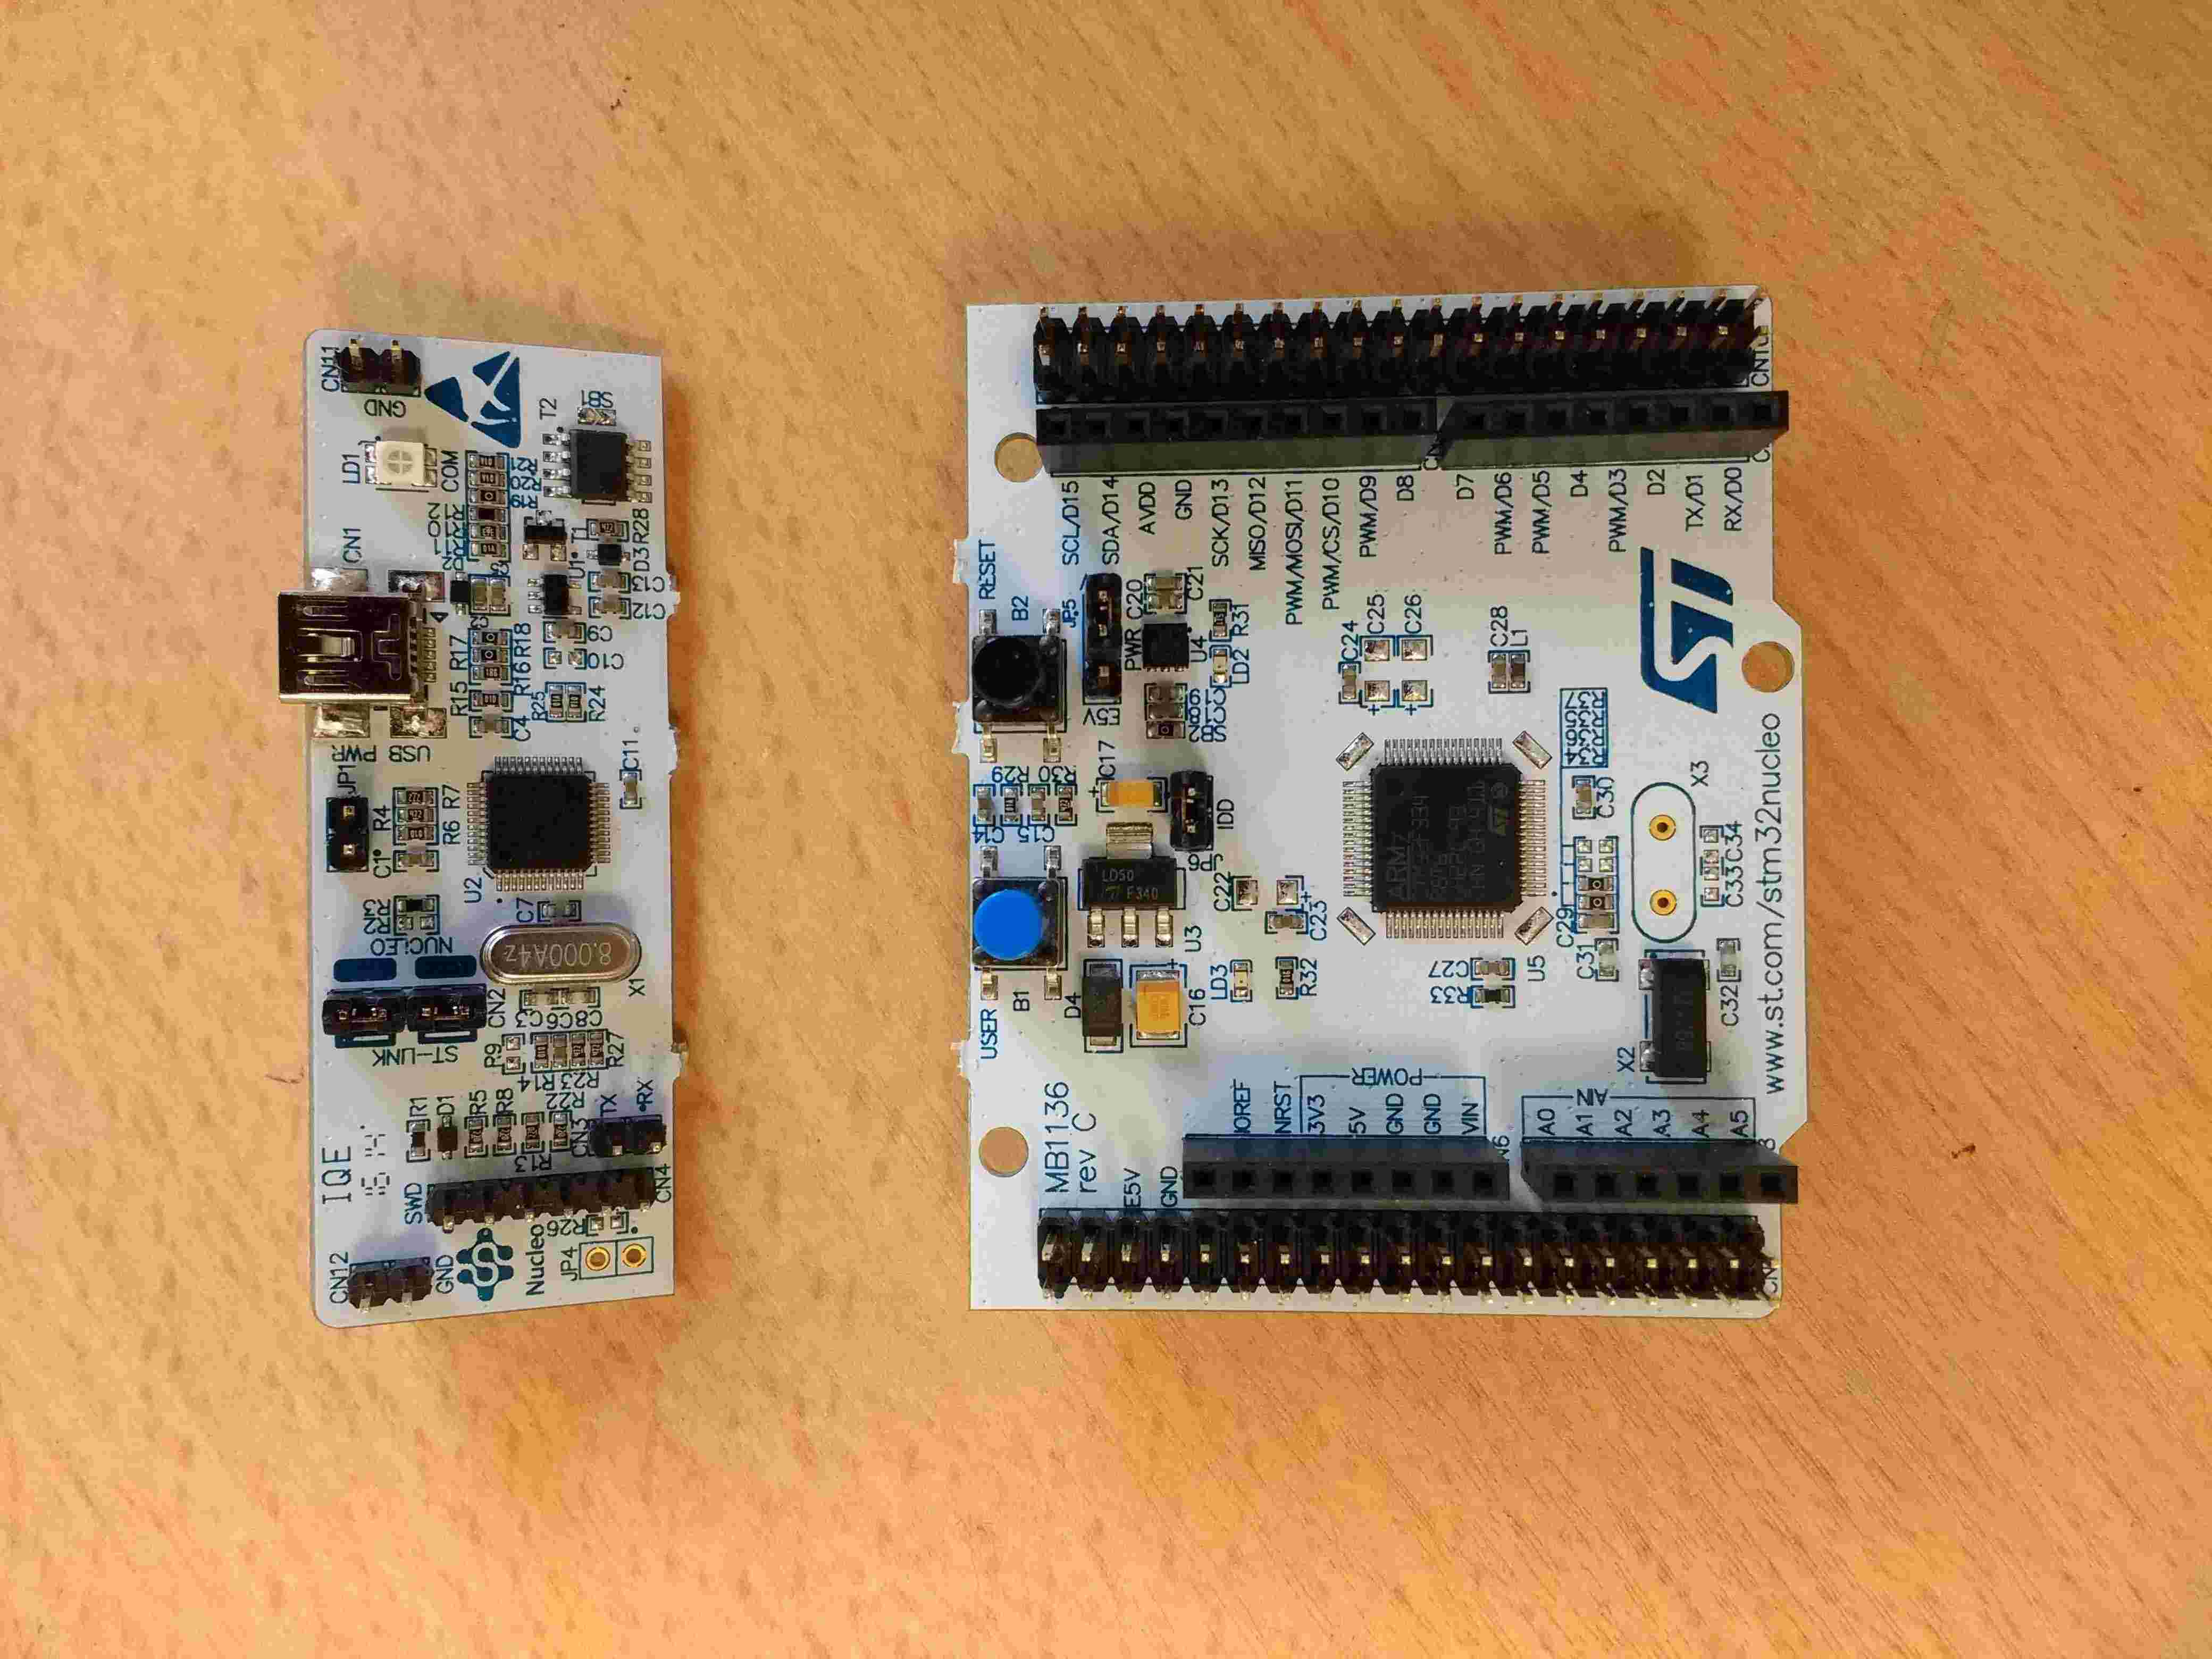
\includegraphics[keepaspectratio=true,scale=0.1]{nucleo_debug.jpg}
\label{visina8}
\end{center}\end{figure}






Connectez le Tag-connect au nucleo selon ce tableau et selon les schémas des connecteurs :



\begin{figure}[H]
\begin{center}
\advance\leftskip-3cm
\advance\rightskip-3cm
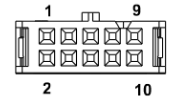
\includegraphics[keepaspectratio=true,scale=1]{tag_connectpinout.png}
\caption{Tag-Connect}
\label{visina8}
\end{center}\end{figure}




\begin{figure}[H]
\begin{center}
\advance\leftskip-3cm
\advance\rightskip-3cm
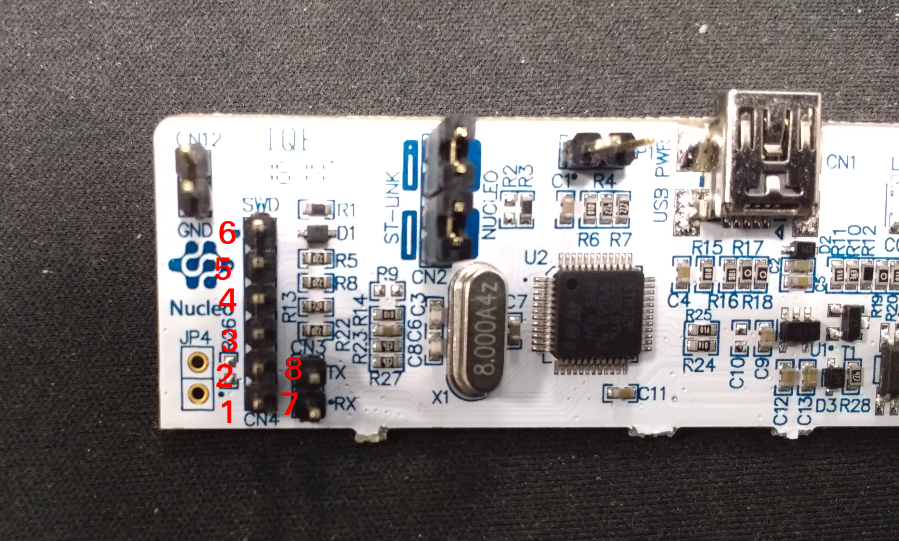
\includegraphics[keepaspectratio=true,scale=0.3]{Nucleo_pins.png}
\caption{Nucleo}
\label{visina8}
\end{center}\end{figure}


\begin{center}
 \begin{tabular}{||c | c | c ||} 
 \hline
 Pin Nucleo  & Pin Tag-Connect \\ [0.8ex] 
 \hline\hline
  6 VDD TARGET   &  1 Vcc \\ 
 \hline
   3 SWDIO & 2 SWDIO \\
 \hline
  4 GND  & 3 Gnd\\
 \hline
  5 SWCLK  &  4 SWCLK\\
 \hline
  X  & X \\ [1ex] 
 \hline
  1 SWO  & 6 SWO \\ [1ex]
 \hline
  7 Rx  & 7 Tx \\ [1ex] 
 \hline
  X  & X \\ [1ex] 
 \hline
 8 Tx & 9 Rx \\ [1ex] 
 \hline
 2 NRST & 10 NRST\\ [1ex] 
 \hline
\end{tabular}
\end{center}





Cela permet de connecter le produit idosens en UART en en SWD au PC.

Connectez le Tag-Connect au Nucleo et alimentez le produit par le module "Power" selon ce schéma :



\begin{figure}[H]
\begin{center}
\advance\leftskip-3cm
\advance\rightskip-3cm
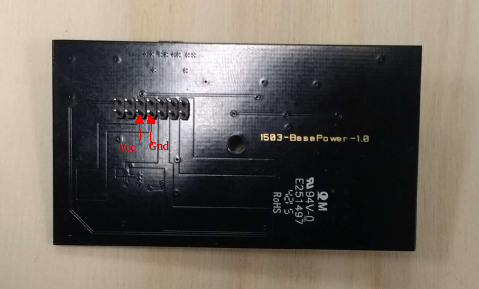
\includegraphics[keepaspectratio=true,scale=0.6]{power_dos_fleches.png}

\label{visina8}
\end{center}\end{figure}

\begin{figure}[H]
\begin{center}
\advance\leftskip-3cm
\advance\rightskip-3cm
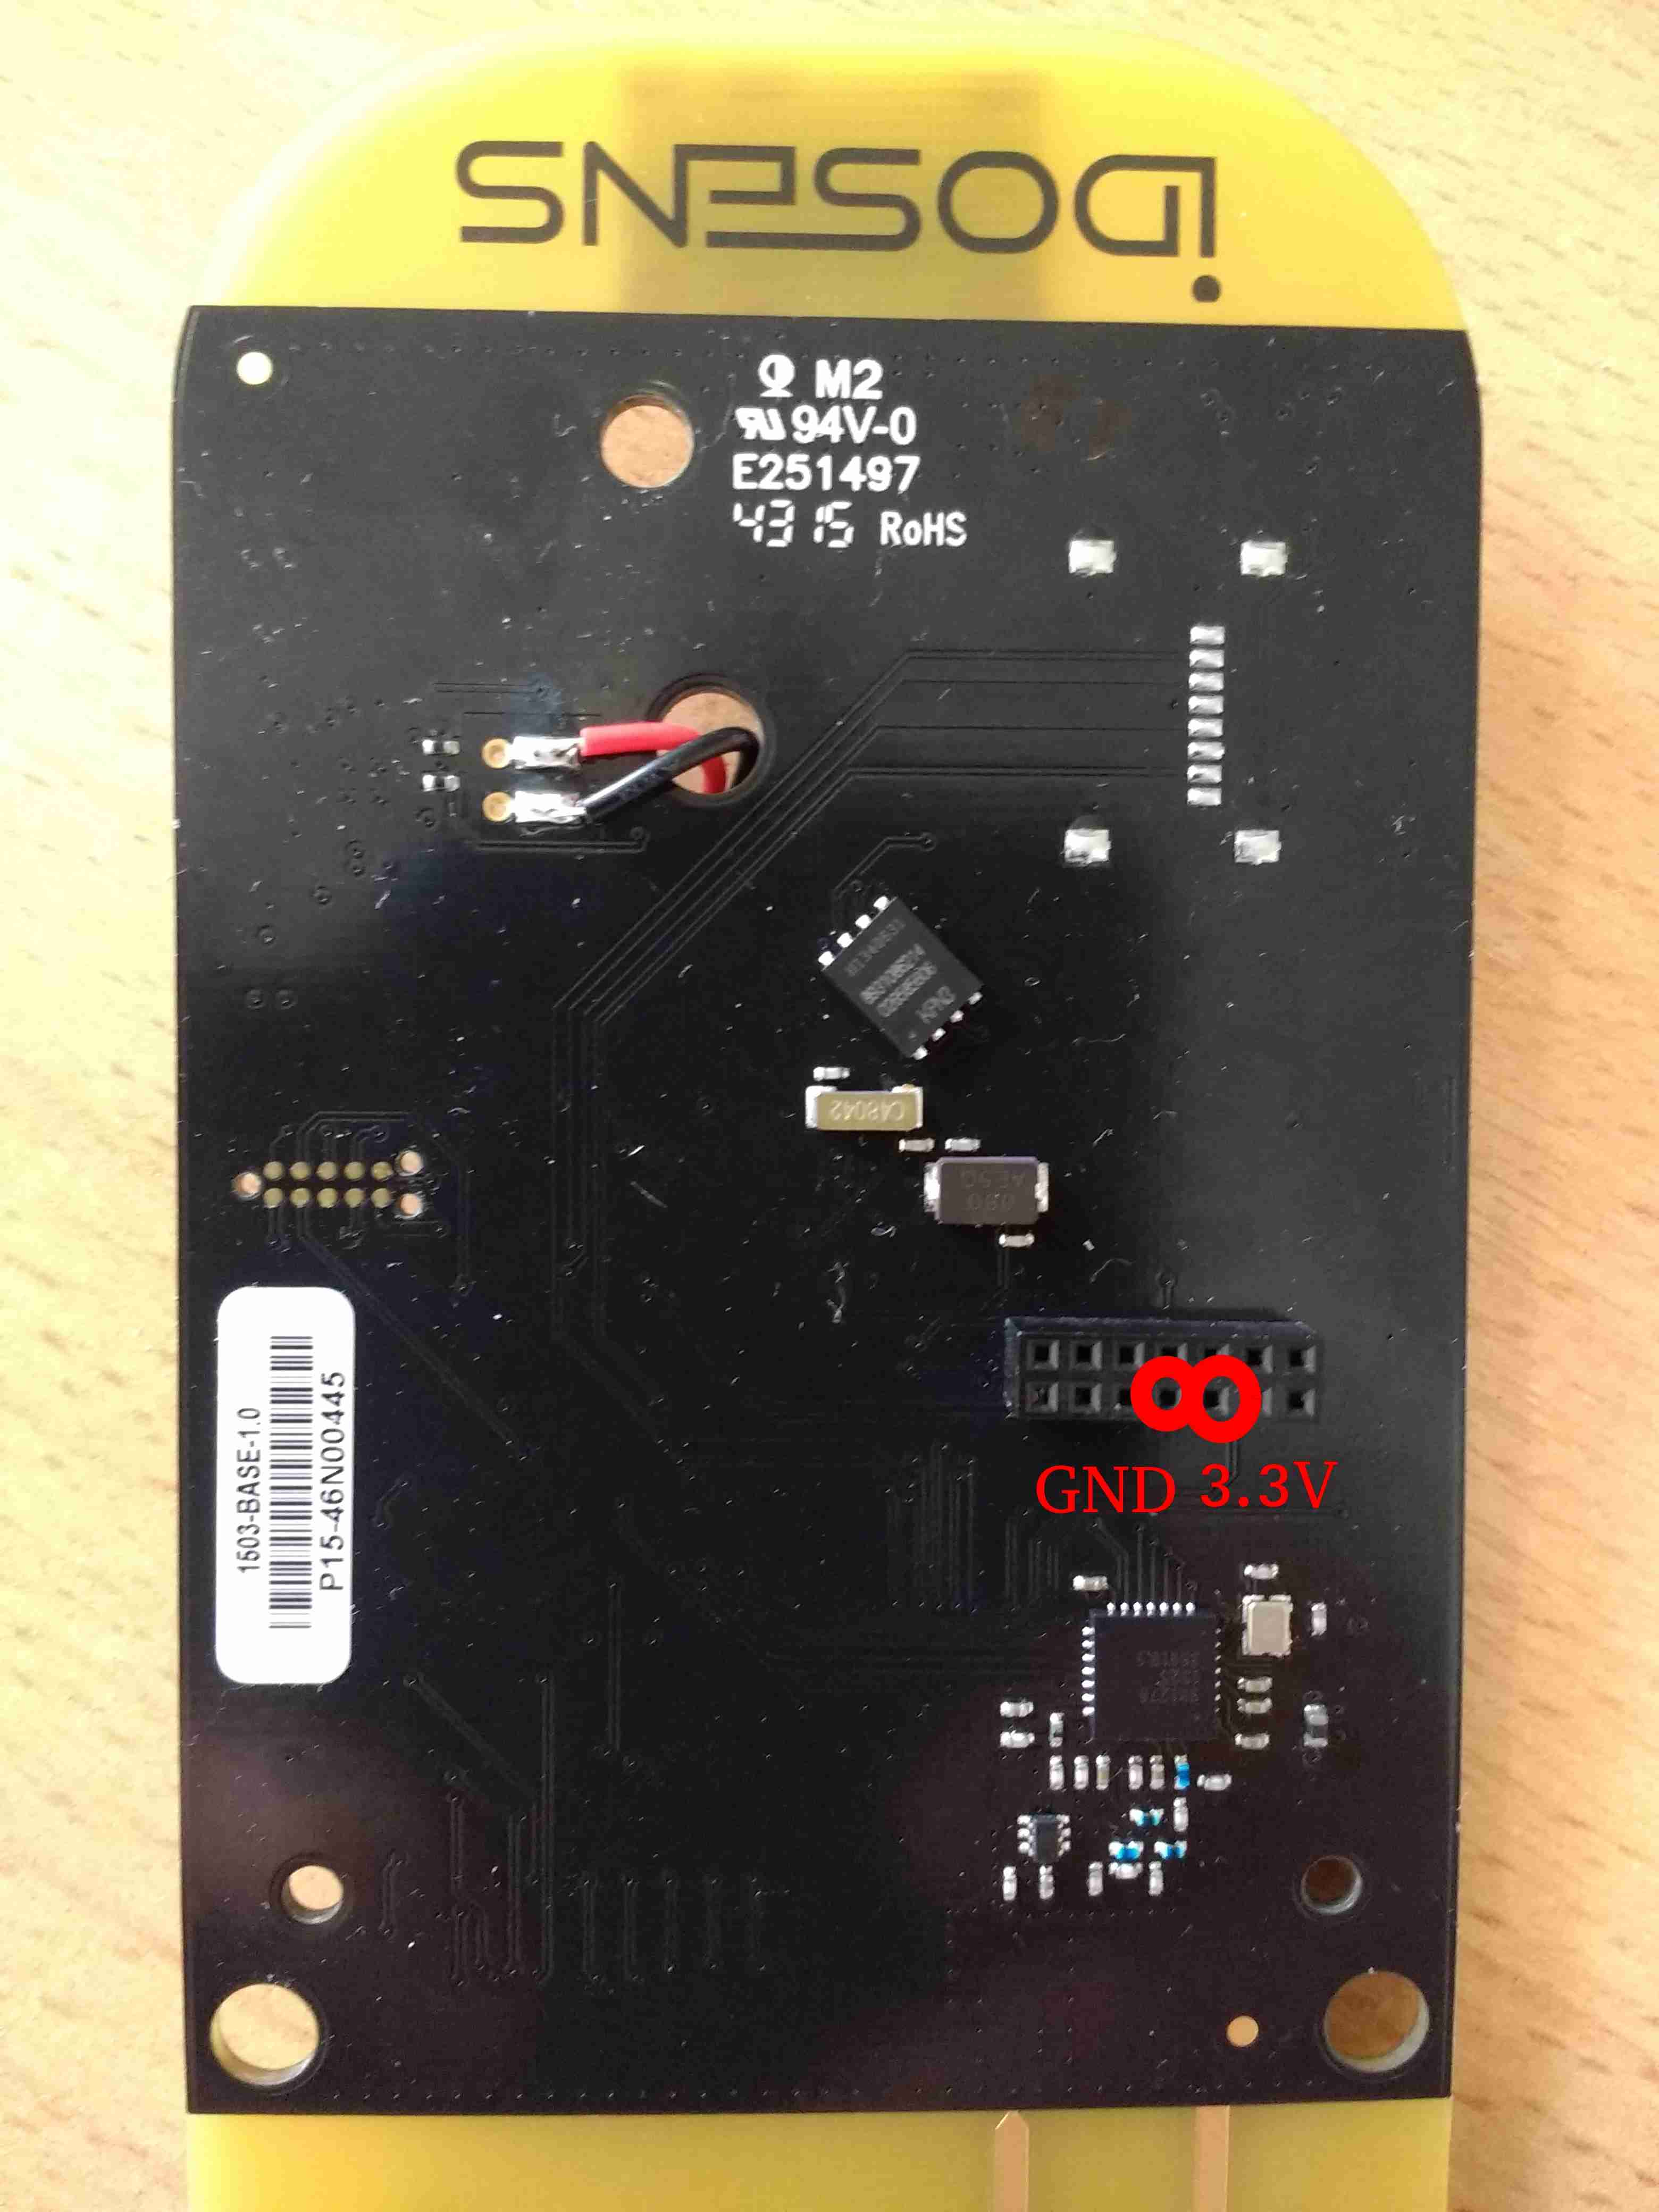
\includegraphics[keepaspectratio=true,scale=0.1]{branchement_basepower2.jpg}

\label{visina8}
\end{center}\end{figure}


Photo du montage :

\begin{figure}[H]
\begin{center}
\advance\leftskip-3cm
\advance\rightskip-3cm
\includegraphics[keepaspectratio=true,scale=0.1]{montage.jpg}

\label{visina8}
\end{center}\end{figure}

\subsection{Flasher le firmware sur le produit}

\subsubsection{Déverouiller le port USB}
Sur Linux : ajoutez un fichier 50-myusb.rules dans 
\begin{minted}{bash}
/etc/udev/rules.d

\end{minted}
contenant 
\begin{minted}{bash}
ACTION=="add", KERNEL=="ttyACM[0-9]*", ATTRS{idVendor}=="0483",
ATTRS{idProduct}=="374b", MODE="0666"

\end{minted}
avec idProduct et idVendor à renseigner en fonction du votre produit. On les trouve avec la commande 
\begin{minted}{bash}
lsusb

\end{minted}

\begin{figure}[H]
\begin{center}
\advance\leftskip-3cm
\advance\rightskip-3cm
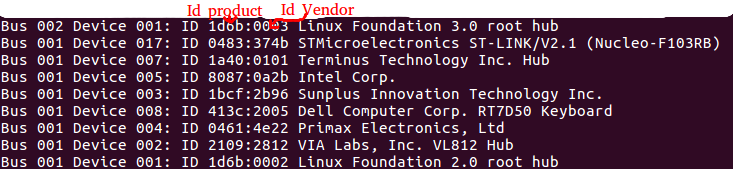
\includegraphics[keepaspectratio=true,scale=0.5]{lsusb2_fleches.png}

\label{visina8}
\end{center}\end{figure}

Redémarrer le PC pour prendre en compte les changements.

Maintenez le Tag-Connect appuyé sur les contacts métallique et cliquez sur le bouton Connect de STM32Cube Programmer :
\begin{figure}[H]
\begin{center}
\advance\leftskip-3cm
\advance\rightskip-3cm
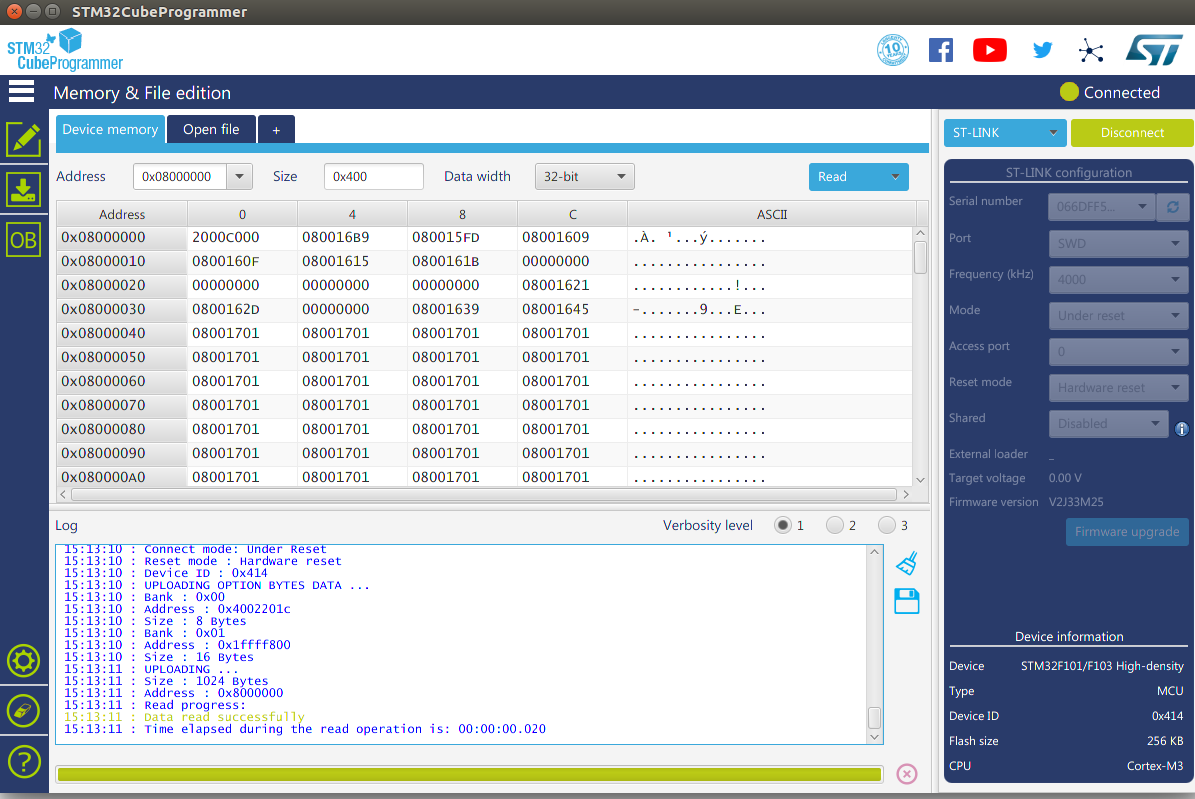
\includegraphics[keepaspectratio=true,scale=0.3]{connected.png}

\label{visina8}
\end{center}\end{figure}

Pour charger le fichier .bin ou .elf souhaité cliquez sur l'onglet "Open file".
Une fois le produit connecté et le firmware sélectionné, appuyé sur le bouton Download toujours en maintnenant appuyé le tag-connect.

\begin{figure}[H]
\begin{center}
\advance\leftskip-3cm
\advance\rightskip-3cm
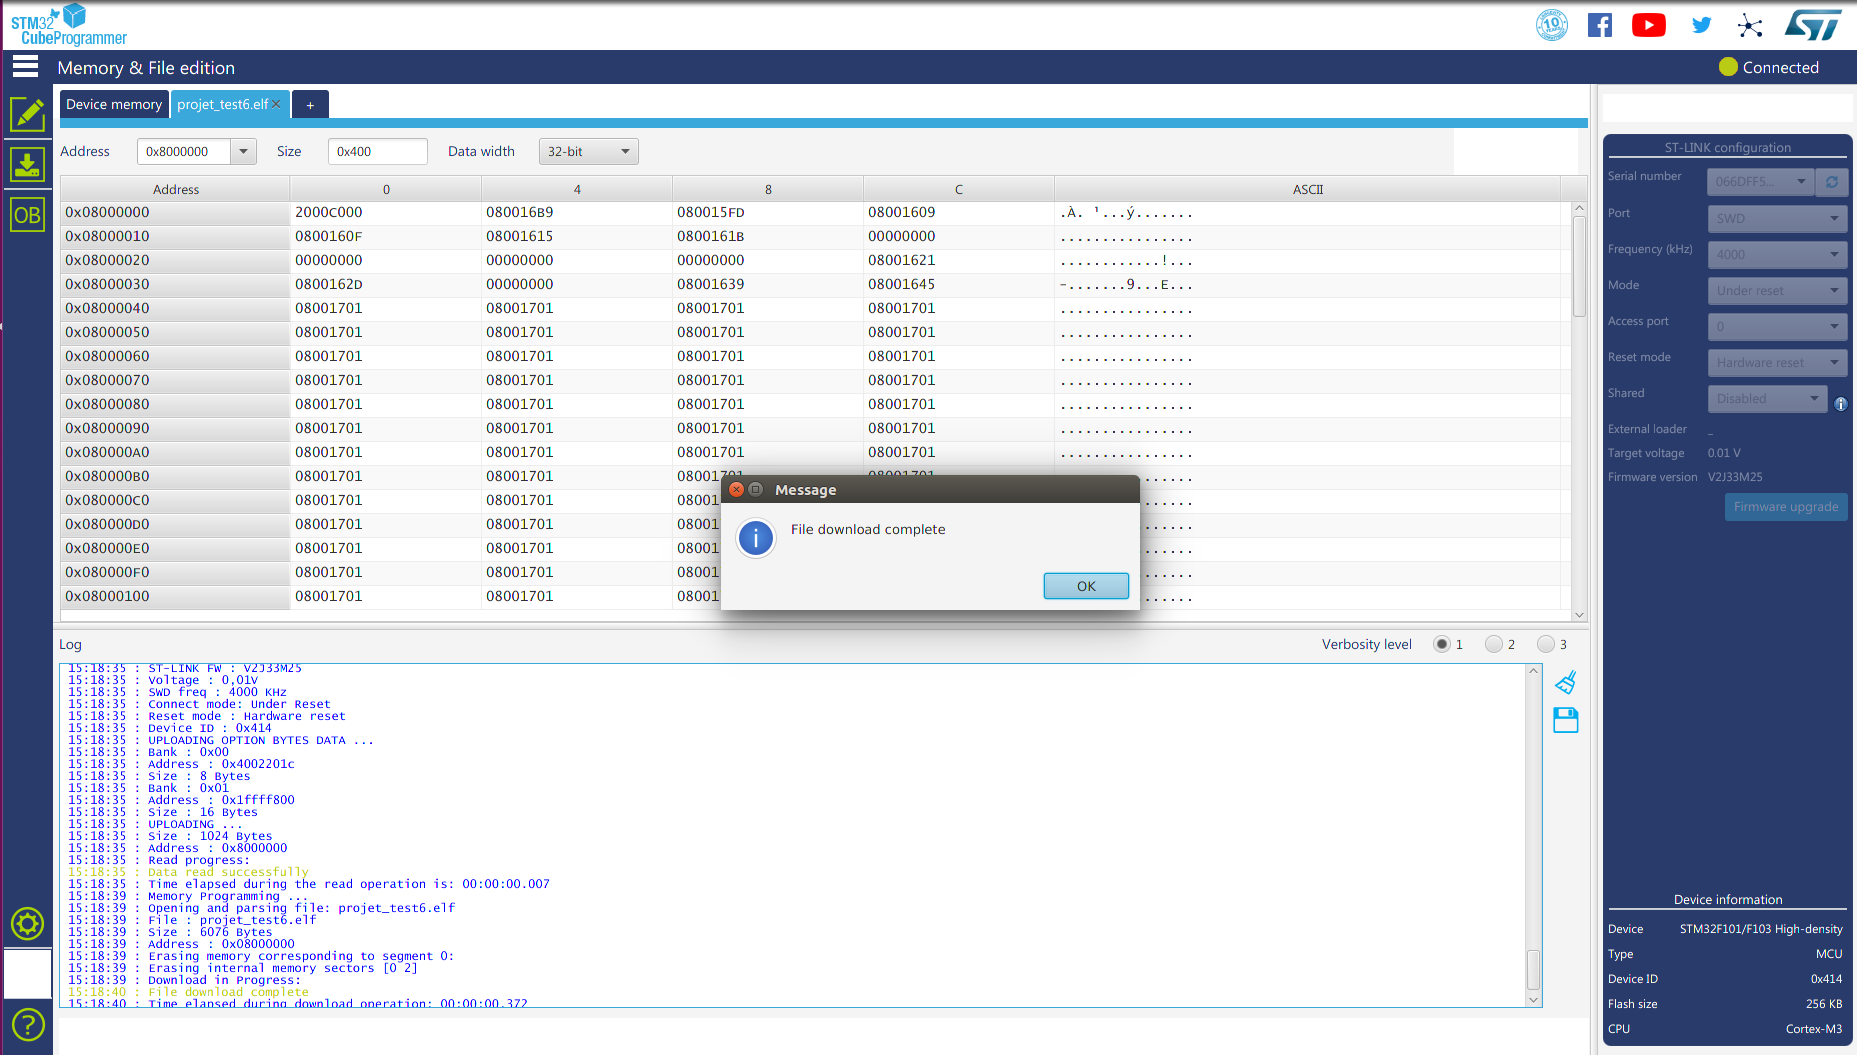
\includegraphics[keepaspectratio=true,scale=0.3]{downloaded.png}

\label{visina8}
\end{center}\end{figure}

\subsection{Reset du produit}
Pour prendre en compte le nouveau firmware, il faut "reseter" le produit en branchant/débranchant l'alimentation du bloc "BasePower".


\section{Résultat}

Débranchez puis rebranchez la carte pour réinintialiser le microcontrôleur.\\
Ouvrez un terminal série comme Putty ou minicom.
Sélectionnez le bon port, dans mon cas sur Ubuntu 16.04 ttyACM0.
Sur Linux, pour connaître le port sur lequel est branché le produit :

\begin{minted}{bash}
ls /dev

\end{minted}

Choisir un baudrate de 115200.


\begin{figure}[H]
\begin{center}
\advance\leftskip-3cm
\advance\rightskip-3cm
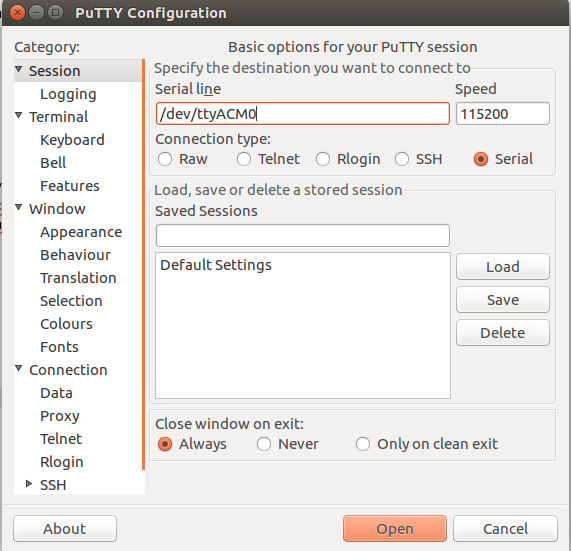
\includegraphics[keepaspectratio=true,scale=0.5]{putty.png}

\label{visina8}
\end{center}\end{figure}


\begin{figure}[H]
\begin{center}
\advance\leftskip-3cm
\advance\rightskip-3cm
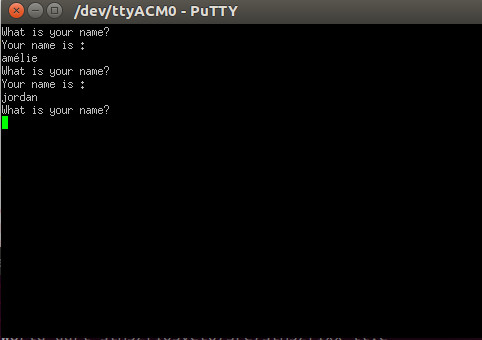
\includegraphics[keepaspectratio=true,scale=0.5]{whatisyourname.png}

\label{visina8}
\end{center}\end{figure}







\end{document}
